\documentclass[11pt, oneside]{report}   	% use "amsart" instead of "article" for AMSLaTeX format
\usepackage[margin = 1in]{geometry}                		% See geometry.pdf to learn the layout options. There are lots.
\geometry{a4paper}                   		% ... or a4paper or a5paper or ... 
%\geometry{landscape}                		% Activate for rotated page geometry
\usepackage[parfill]{parskip}    		% Activate to begin paragraphs with an empty line rather than an indent
\usepackage{graphicx}				% Use pdf, png, jpg, or eps§ with pdflatex; use eps in DVI mode
								% TeX will automatically convert eps --> pdf in pdflatex	
\usepackage{subcaption}									
\usepackage{amsfonts, amsmath,amssymb}
\usepackage{siunitx}
\usepackage[none]{hyphenat}
\usepackage{fancyhdr}
\usepackage{setspace}
\usepackage{hyperref}
%\usepackage[nottoc, notlot, notlof]{tocbibind}		%table of contents
\usepackage{helvet}
\renewcommand{\familydefault}{\sfdefault}

\usepackage{wrapfig}

\usepackage{multirow}
\usepackage[table,xcdraw]{xcolor}
\usepackage{array}
\newcolumntype{L}{>{\centering\arraybackslash}m{7cm}}

\usepackage{csquotes}

\usepackage{epstopdf}
\DeclareGraphicsExtensions{.pdf,.png,.jpg,.eps}

\usepackage{titlesec}
%\titlespacing\chapter{0pt}{4pt plus 4pt minus 2pt}{4pt plus 2pt minus 2pt}
\titlespacing\section{0pt}{4pt plus 4pt minus 2pt}{0pt plus 2pt minus 2pt}
\titlespacing\subsection{0pt}{4pt plus 4pt minus 2pt}{0pt plus 2pt minus 2pt}
\titlespacing\subsubsection{0pt}{4pt plus 4pt minus 2pt}{0pt plus 2pt minus 2pt}

\titleformat{\chapter}[display]
{\normalfont\huge\bfseries}{\chaptertitlename\ \thechapter}{0pt}{\Huge}
\titlespacing*{\chapter}{0pt}{0pt}{0pt}

\usepackage{sidecap}

\pagestyle{fancy}
\fancyhead{}
\fancyfoot{}
\fancyhead[L]{\slshape \MakeUppercase{4YP Report}}
\fancyhead[R]{\slshape 355136}
\fancyfoot[C]{\thepage}
%\renewcommand{\headrulewidth}{0pt} %remove line in header

\setlength{\parskip}{1em}
\doublespacing

% alternative margin for declaration page
\newenvironment{changemargin}[3]{%
\begin{list}{}{%
\setlength{\topsep}{0pt}%
\setlength{\leftmargin}{#1}%
\setlength{\rightmargin}{#2}%
\setlength{\topmargin}{#3}%
\setlength{\listparindent}{\parindent}%
\setlength{\itemindent}{\parindent}%
\setlength{\parsep}{\parskip}%
}%
\item[]}{\end{list}}


\usepackage{mathtools}
\newcommand\SmallMatrix[1]{{%
  \big\arraycolsep=0.5\arraycolsep\ensuremath{\begin{pmatrix}#1\end{pmatrix}}}}
\DeclareMathOperator{\diag}{diag}
%\DeclareMathOperator{\f}{f}

\renewcommand{\vec}[1]{\mathbf{#1}}


\title{B1 Project Report}
\author{Candidate Number: 355136}
\date{}							% Activate to display a given date or no date

\begin{document}
\pagenumbering{Roman}

\begin{titlepage}
\begin{center}
\vspace*{1cm}
\Large {\textbf{The University of Oxford}}\\
\Large{\textbf{Engineering Science}}\\
\vfill
\noindent\rule{5in}{0.6pt}\\[1mm]
\huge{\textbf{4YP Project Report}}\\[3mm]
\Large{\textbf{- Using Machine Learning to Control Software Synthesisers  -}}\\[1mm]
\noindent\rule{5in}{0.6pt}\\[1mm]
\vfill
Candidate Number: 355136\\
\today\\
\end{center}
\end{titlepage}

%\newgeometry{left=0cm,right=0cm,top=0cm,bottom=0cm}
\begin{changemargin}{-1in}{0in}{-1.5in}

\includegraphics{Declaration_of_Authorship_form_2018.pdf}
\thispagestyle{empty}
\end{changemargin}

\begin{abstract}
\begin{flushleft}
Software Synthesisers (Soft-Synths) are computer applications which create sounds in response to musical input typically in the form of MIDI messages. They are widely used in a variety of musical contexts. Typical soft-synths have hundreds or thousands of parameters which control the sound generation algorithm, allowing the user to create sounds that suit their musical needs. This results in a high dimensional, non-linear search space which the user must navigate in order. Research indicates that humans are bad at navigating such interfaces with serial controls, and that there is a strong link between interface design and the level of creativity that the user with experience when using the interface. \\
This work describes a novel interface designed to help users control synthesisers in a quicker and more intuitive manner. It combines 3 interfaces together: a traditional 'knob and slider' interface, a search space visualisation interface, and an iterative blending interface.

THIS ABSTRACT NEEDS A LOT MORE WORK, WILL WORK ON AFTER WRITING MORE OF THE REPORT
\end{flushleft}
\end{abstract}


%\newgeometry{left=1in,right=1in,top=1in,bottom=1in}
\tableofcontents
%\thispagestyle{empty}
\clearpage
\pagenumbering{arabic}
\setcounter{page}{1}


%%%%%%%%%%%%%%%%%%%%%%%%%%%%%%%%%%%%%%%%%%%%%%%%%%%%%%%%%%%%%%%%%%%%%%%%%%%%%
\chapter{Introduction}
%\section{Background Information}
Software Synthesisers (Soft-Synths) are computer applications which create sounds in response to musical input typically in the form of MIDI (\emph{Musical Instrument Digital Interface}) messages. They are widely used in a variety of musical contexts. Typical soft-synths have hundreds or thousands of parameters which control the sound generation algorithm, allowing the user to create sounds that suit their musical needs. This results in a high dimensional, non-linear search space which the user must navigate in order. Research indicates that humans are bad at navigating such interfaces with serial controls, and that there is a strong link between interface design and the level of creativity that the user with experience when using the interface \cite{TubbThesis}. \\
This work describes a novel interface designed to help users control synthesisers in a quicker and more intuitive manner. It combines 3 interfaces together: a traditional 'knob and slider' interface, a search space visualisation interface, and an iterative blending interface.

A video of the full interface being used can be viewed at (LINK TO VIDEO).
\section{Aims of the project}
\begin{itemize}
	\item Create a synthesiser to test the interface with.
	\item Create dataset of synthesiser presets
	\item Create low dimensional embedding of the preset dataset
	\item Prototype the user interface (UI).
	\item Determine an optimal way to generate new presets for each  iteration of the Blending INterface
\end{itemize}
NEEDS WORK
\section{Methodology}
The main methodology taken in this project is that the set of preset sounds for a synthesiser contain a lot of useable information. This is because much of the parameter space of typical synthesisers creates inaudible, or terrible sounding sounds, and the presets have been designed to avoid such regions, and to highlight a diverse range of the synth's best sounds. By working to map the timbre of the presets, rather than the timbre of the entire parameter space, a much simpler, and hopefully more useful latent space can be identified, only requiring simpler statistical techniques to be used.

The project is aimed at fixed architechure parmetric synhesisers, such as FM, additive, subractive, and physical modelling synthesisers.
NEEDS MORE WORK.
\chapter{Literature Review}
\section{Introduction to Synthesisers}
Synthesisers are devices which can create a wide waviety of musical sounds in response to  user input, typically in the form of notes played on a keyboard. %The first synthesisers consisted of single note electronic oscilators, such as the Theremin... , 
Wiki - "The earliest synthesizers used a variety of thermionic-valve (vacuum tube) and electro-mechanical technologies.". \\
In the 1960s and 70s, after the invention of the transistor, - Wiki - "Early analog synthesizers used technology from electronic analog computers and laboratory test equipment. They were generally "modular" synthesizers, consisting of a number of independent electronic modules connected by patch cables into a patchbay that resembled the jackfields used by 1940s-era telephone operators. Synthesizer modules in early analog synthesizers included voltage-controlled oscillators (VCOs), voltage-controlled filters (VCFs), and voltage-controlled amplifiers (VCAs). The control voltage varied frequency in VCOs and VCFs, and attenuation (gain) in VCAs. Additionally, they used envelope generators, low-frequency oscillators, and ring modulators. Some synthesizers also had effects devices, such as reverb units, or tools such as sequencers or sound mixers. Because many of these modules took input sound signals and processed them, an analog synthesizer could be used both as a sound-generating and sound-processing system.\\
Famous modular synthesizer manufacturers included Buchla \& Associates, Moog Music, ARP Instruments, Inc., and Electronic Music Studios."
Later analogue synths were fixed architecture (or semi-modular), and much more compact and user friendly. -Wiki- "The most popular of these was the Minimoog". At this time, synthesisers began to feauture commoonly in popular music, both in the studio and in live situations.\\
In the 1980s, digital syntheisers were invented, allong with a much wider variety of syntesis techniques than was possible with analogue electronics. In particular FM synthesis defined much of the musical sound of the 1980s, and was poularised by the Yamaha DX7 synthesisers. (REFERENCE ALL THIS STUFF!)

Since the invention of personal computers, many popular synthesisers have been recreated digitally as software synthesisers, commonly known as 'Plug-ins', and are widely used in modern Digital Audio Workstations (DAWs). As well as recreatations of hardsware synthesisers, many novel software synthesisers have been developed solely for use on computers, making use of the flexibility, the increased computing power, and interactive display capabitilies of computers. 

In the thesis "Development and Exploration of a Timbre Space Representation of Audio" \cite{SynthTypes} %http://mig.dcs.gla.ac.uk/wp-content/mig-papers/craig_nicol_thesis.pdf
the common methods of audio synthesis are decrebed in detail, and are as follows:
\begin{itemize}
	\setlength\itemsep{-1.2em}
	\item Wavetable Synthesis
	\item Synthesis using Oscillators
	\item Additive Synthesis
	\item Frequency Modulation (FM) Synthesis
	\item Subtractive Synthesis
	\item Granular Synthesis
	\item Physical Modelling
\end{itemize}
In addition, many synthesisers inlcude the use of audio samples. Hybrid approcaches of the above techniques are also common.

\section{Introduction to Synthesiser Interfaces}
Analogue synthesiser interfaces, whether modular or fixed architecture, usually consist of a number of modules, such as VCOs and VCAs, controlled with potentiometers, switches, and control signals from elsewhere in the synth, see Figure \ref{fig:MoogSystem35}. \\
%
\begin{figure}[h] 
	\centering
	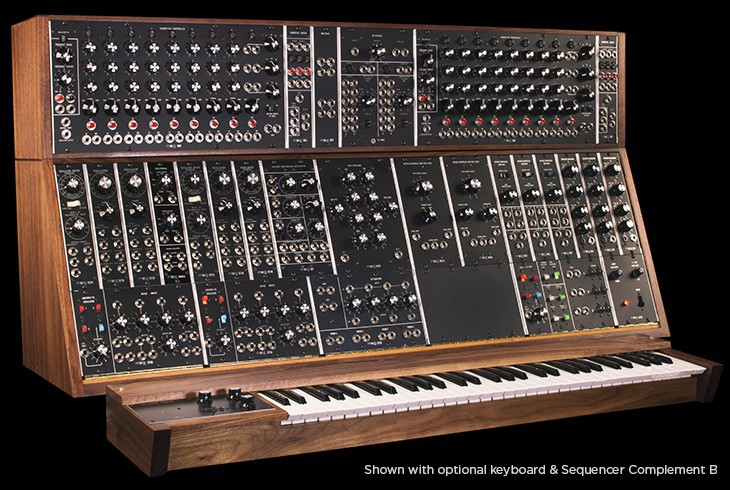
\includegraphics[width = 6in]{MoogSystem35.jpg}
	\caption{Analogue synthesiser - Moog System 35}
	\label{fig:MoogSystem35}
	% https://www.moogmusic.com/products/modulars/system-35
\end{figure}
%
Digital synthesisers can be much more flexible in their interface, as the audio signals are not passing directily thorugh the controls. Early digital synthesisers had famously un-user friendly interfaces comsising of LCD screens and rows of buttons to alter the parameters, hidden in a series of menus, see Figure \ref{fig:YamahFS1R}. As these interfaces lacked the 'hands-on' interface that musicians loved from analogue synths, many digital synths, despite being much more capable of producing a wide variety sounds, were less popular than analogue synths, and many users found the process of programming these synths to be incredibly frustrating. (REFERENCE FOR THIS) To make the intefaces more user friendly, most digital synths are provided with a set of 'Presets' - parameter settings that produce 'nice' sounds - which demonstarate a wide range of the synthesiser's sounds. One of the reasons the synthesiser sounds of the 1980s were so simlar to each other, is that many musicians would entirely use the preset sounds, without altering them at all. This is in part due to the novely of the sounds at the time, and in part due to the difficult user interfaces.\\
%
\begin{figure}[h] 
	\centering
	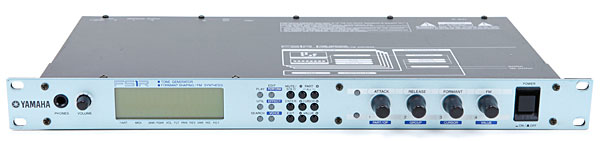
\includegraphics[width = 6in]{yamaha_fs1r.jpg}
	\caption{Digital synthesiser - Yamaha FS1R}
	\label{fig:YamahFS1R}
	% http://www.vintagesynth.com/yamaha/fs1r.php
\end{figure}
Software synthsesiers have a wide variety of interfaes. Many follow similar design patterns to analogue synths, but with additional interactive elements such as 'user drawable' envelopes. An example of this is the very popular Massive by Native Instruments, shown in Figure \ref{fig:MassiveNI}. Other software synthesisers offer musch more visual and interactive interfaces, such as the Ableton Wavetable synthesiser, shown in Figure \ref{fig:AbletonWavetable}.

\begin{figure}[h] 
	\centering
	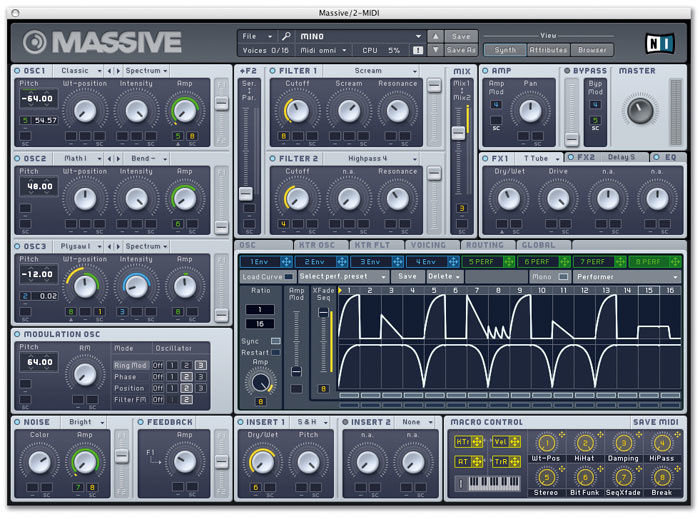
\includegraphics[width = 6in]{MassiveNI.jpg}
	\caption{Software Synthesiser - Massive (Native Instruments) }
	\label{fig:MassiveNI}
	%https://www.soundonsound.com/reviews/native-instruments-massive
\end{figure}

\begin{figure}[h] 
	\centering
	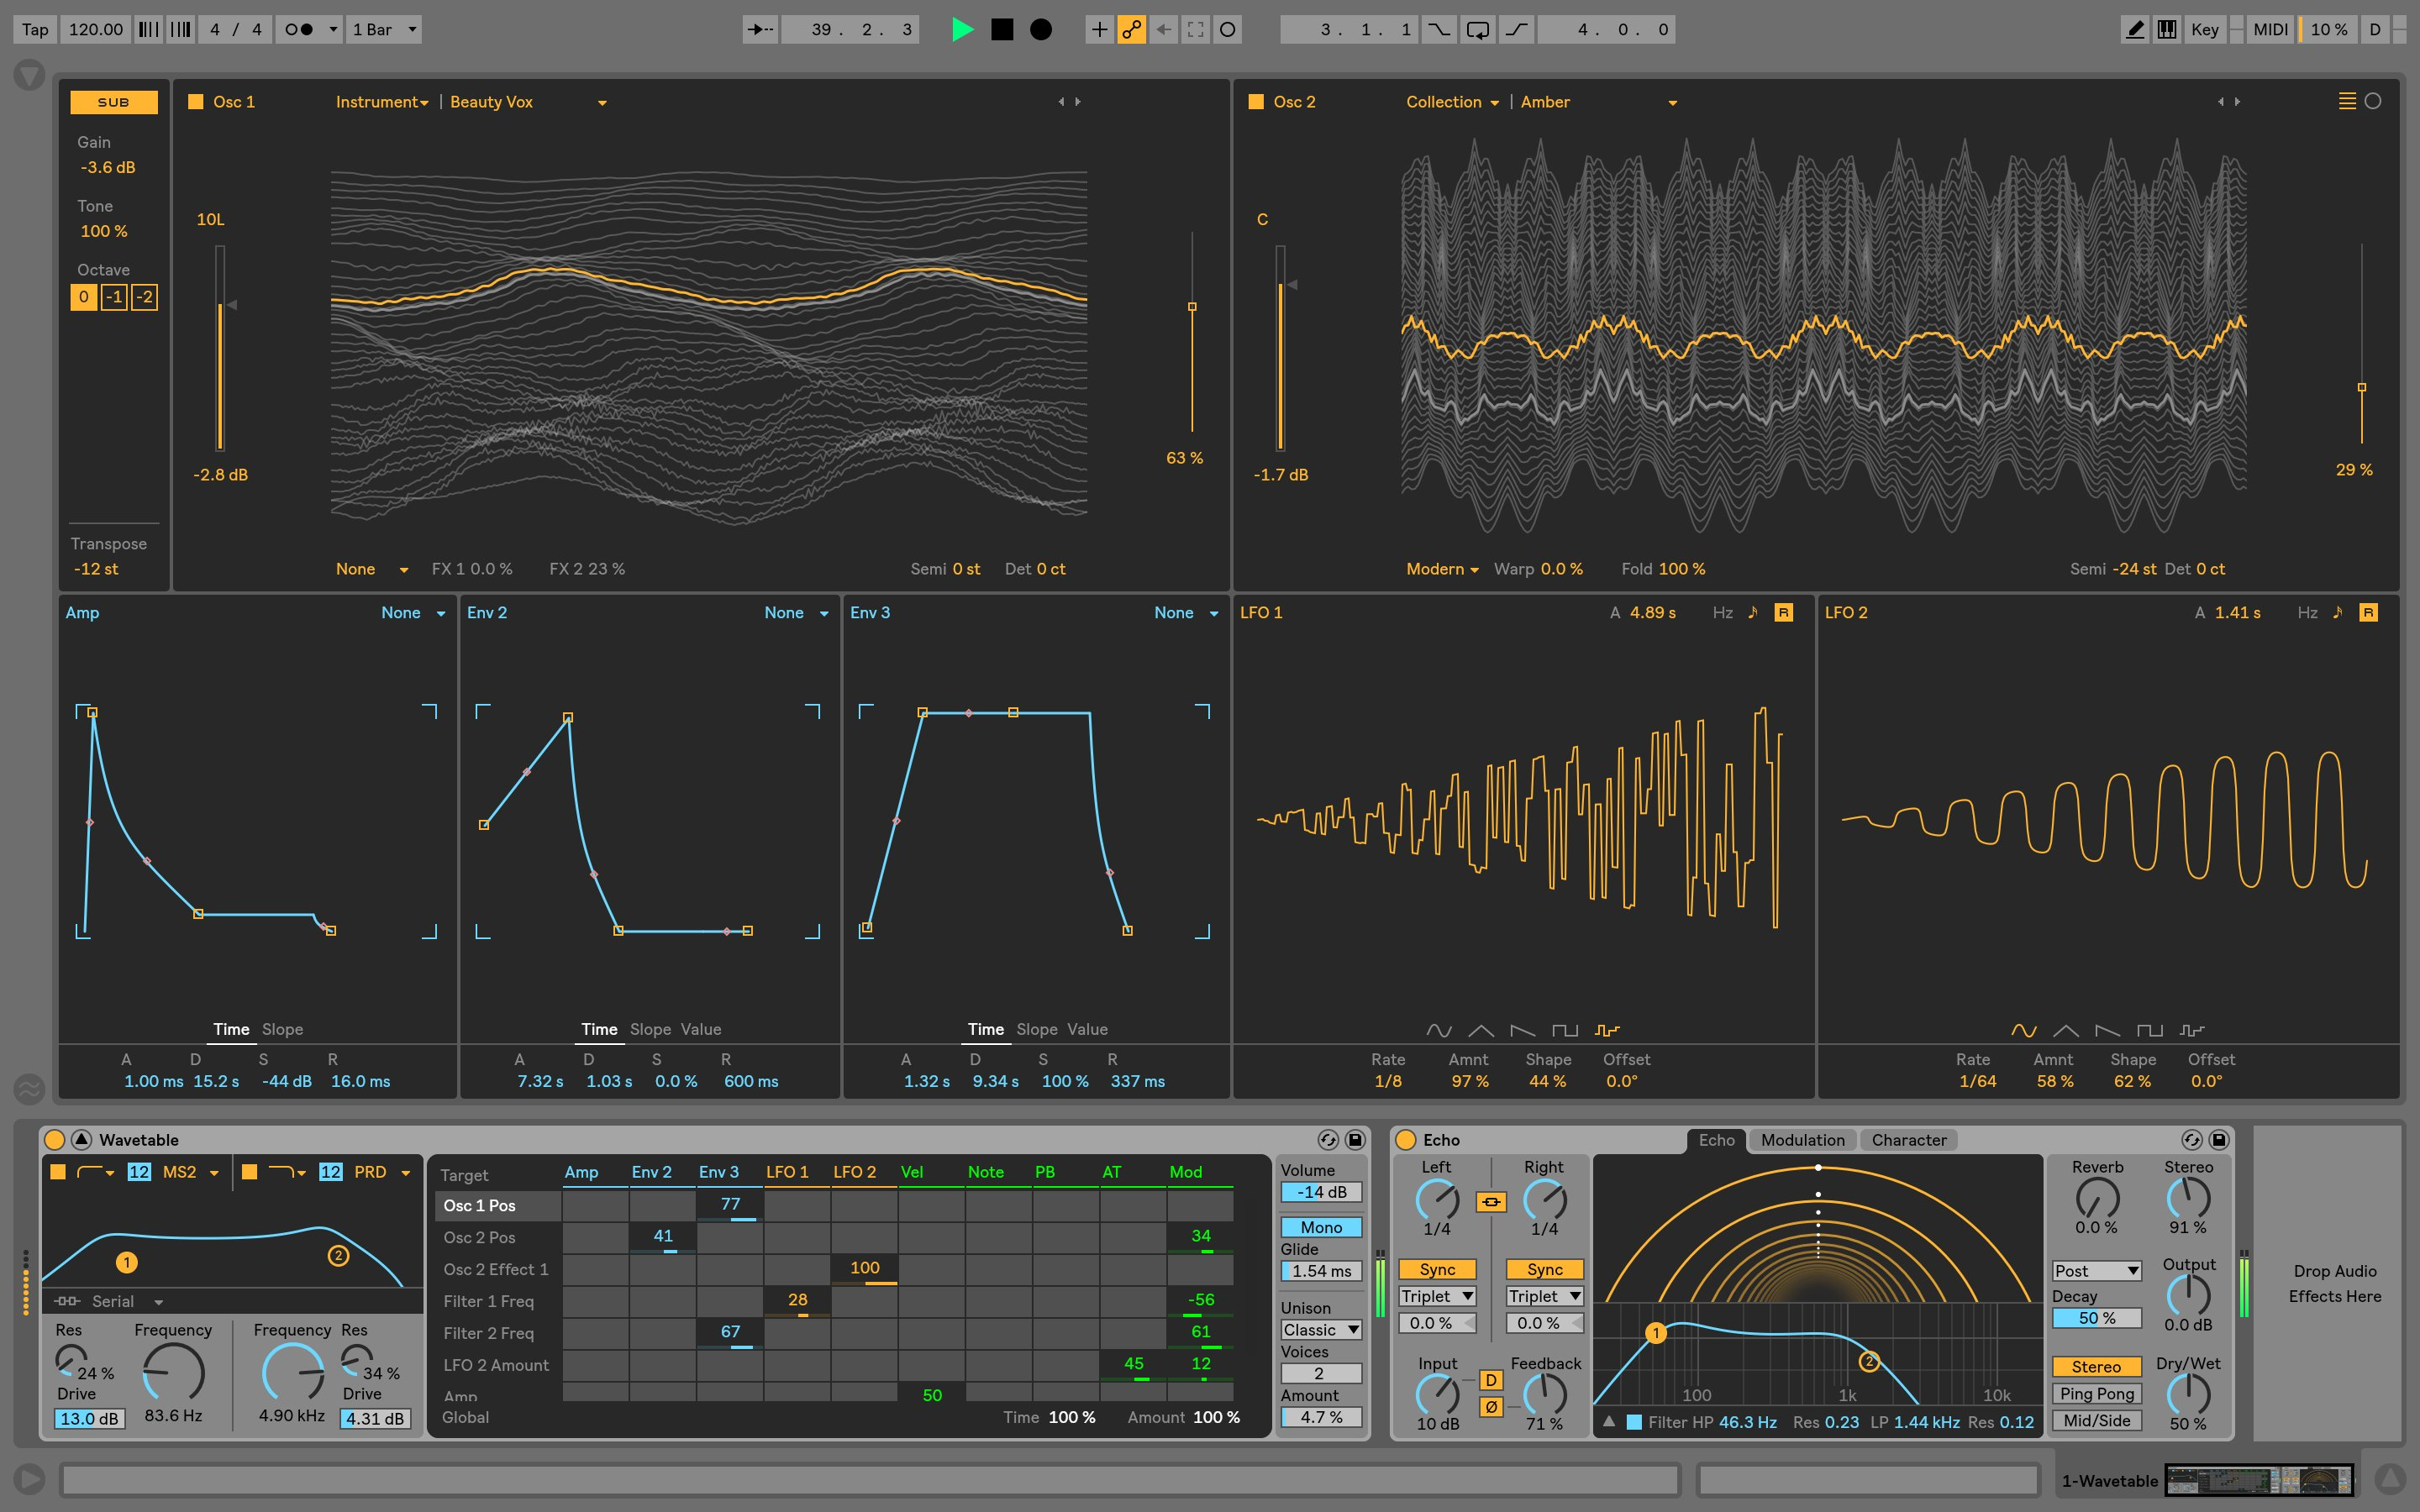
\includegraphics[width = 6in]{AbletonWavetable.jpg}
	\caption{Software Synthesiser - Wavetable (Ableton) }
	\label{fig:AbletonWavetable}
	%https://www.ableton.com/en/packs/wavetable/
\end{figure}

Some software synthesisers have modular designs, such as SoftTube Modular, and some even allow users to program synthesis modules from scratch, such as Max/MSP and Supercollider.

There has been lots of reasearch in the Computer Music field to use multideminsional controllers, such as the Myo, Leap Motion and Microsoft Kinect, to control synthesis parameters in real time, and research into advanced user interaction types, such as preset blending and randomisation of presets. (EXAMPLES!!) Several studies have applied a variety of machine learning techniques to synthesiser control, as described in the next section.

\section{Previous attempts of using machine learning to control synthesisers}
NEEDS A LOT OF WORK!!\\
There have been several previous attempts to use machine learning to make programming synthesisers easier and more expressive.

Talk about the preset blending study, including the parameter freezing.

Talk about automatic tone matching \cite{YeeKing}

Talk about the google sample mapping with TSNE (infinite drum machine). The Selection Interface draws inspiration from this project.

Talk about how taking a sound sample from each preset could be a good way to do the dimensionality reduction interface, but how a parameter based approach is preferable in many ways. Mention which sound metrics would be good to use, and the difficulties involved. \cite{YeeKing}

Talk about the Wekinator stuff

\section{Description of HCI design principles for creative musical interfaces}\label{sec:Tubb}
NEEDS SOME WORK - most likely needs to be shortened.\\
In the work 'Creativity, Exploration and Control in Musical Parameter Spaces' by Robert H. Tubb \cite{TubbThesis}, the representation and mapping of musical paramers is considered in Section 4.3.

\begin{displayquote}
The principal distinctions between types of mappings are as follows [Hunt et al., 2000].
\begin{itemize}
\setlength\itemsep{-1.2em}
\item One-to-many: one control dimension is mapped to many synthesis parameters.
\item Many-to-one: many control parameters affect one synth parameter.
\item Many-to-many: a combination of the above (known as ‘complex’ map- pings).
\end{itemize}

[Hunt and Kirk, 2000] Complex many-to-many mappings appear to be more effective for expressive performance, and may lead to greater performance improvements with practice. This may seem counterintuitive, as a complex mapping would appear to be less understandable or predictable than the alternative.
“The sliders interface, whilst it physically allowed people to control multiple parameters, forced the user to mentally ‘strip apart’ the control task into separate control streams. This caused a form of cognitive overload which users generally found restricting and frustrating.”
[Hunt and Wanderley, 2002]
\end{displayquote}

A number of guidelines for creative musical interfaces are presented:
\begin{displayquote}
\begin{enumerate}
\setlength\itemsep{-1.2em}
	\item \emph{Low dimensionality}: Control devices often have fewer parameters than synthesis engines. Given the brain’s limited conscious multi-tasking abilities and working memory capacity, simple controllers are preferable.
	\item \emph{Locality}, or distance preservation: Having travelled a certain distance in control space, we want that to be reflected in the distance travelled in parameter space, and ideally perceptual distance too.
	\item \emph{Revisitability}: If we return to the same point, we wish it to sound the same. The location of preset points should be stable.
	\item \emph{Continuity}: If a point is adjacent to another point on the low-dimensional surface, they should be adjacent in the high-dimensional space.
	\item \emph{Smoothness}: Continuous higher derivatives are desirable to eliminate sudden changes in direction, this has relevance to the predictability of a control.
	\item \emph{Linearity}: When a gesture, such as a scroll, occurs it will have a certain effect on that sound, more extreme versions of this gesture should produce more of the same effect. This property is hard to achieve with any dimensionality reduction method, however smoothness implies some linearity in the immediate neighbourhood.
\end{enumerate}
\end{displayquote}
The Blending Interface described in Section \ref{sec:BlendingDescription} follows all of these design guidelines, and the Selection Interface follows all except the \emph{Smoothness} condition (due to the sudden jumps between presets). Both are complex many-to many interfaces.

In the thesis, the EARS model for creative cognition is developed, described in Figure \ref{fig:EARSmodel}. Detailed decriptions of the four quadrants of the model can be found in the thesis, Section 5.5.3
\begin{figure}[h] 
	\centering
	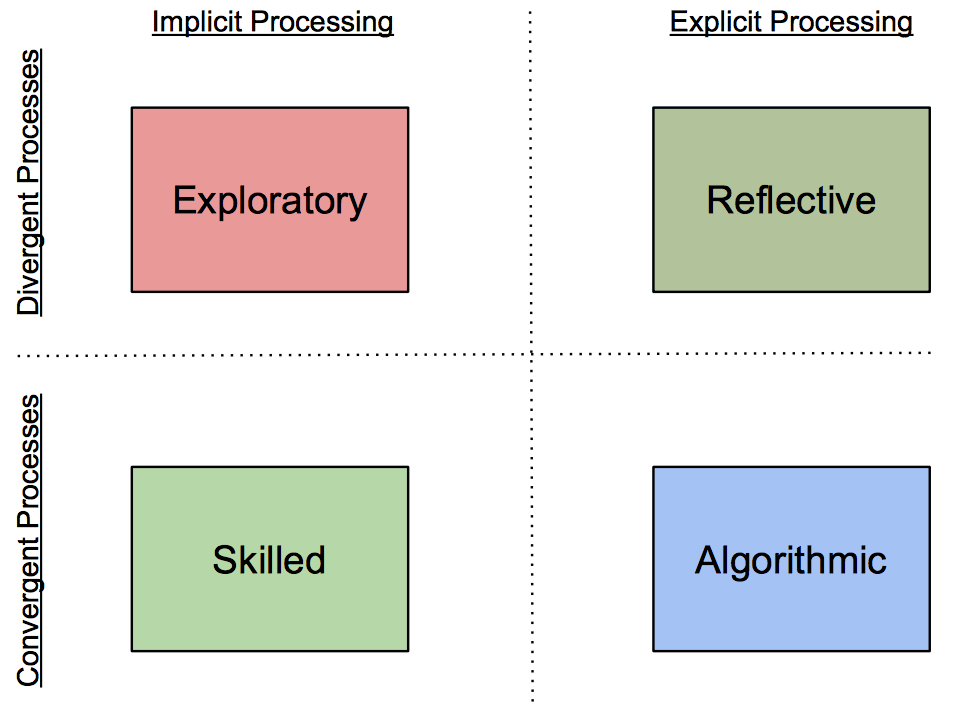
\includegraphics[width = 6in]{EARSmodel.png}
	\caption{The four quadrants formed by drawing distinctions between implicit vs. explicit thinking (left/right) and divergent vs. convergent thinking (top/bottom). (REFERENCE)}
	\label{fig:EARSmodel}
\end{figure}
This project's interface will be evaluatied with this model in Section \ref{sec:EARS}.

%ALSO>>>>>Talk about the stuff about multidemsional controlers having higher thoroughput. - Not sure this is relevant
\section{Principal Component Analysis}
Wiki quote: FIND BETTER SOURCE OR WRITE OWN

"Principal component analysis (PCA) is a statistical procedure that uses an orthogonal transformation to convert a set of observations of possibly correlated variables into a set of values of linearly uncorrelated variables called principal components. If there are $n$ observations with $p$ variables, then the number of distinct principal components is $\min(n−1, p)$. This transformation is defined in such a way that the first principal component has the largest possible variance (that is, accounts for as much of the variability in the data as possible), and each succeeding component in turn has the highest variance possible under the constraint that it is orthogonal to the preceding components. The resulting vectors are an uncorrelated orthogonal basis set. PCA is sensitive to the relative scaling of the original variables."

%In this report, the MATLAB nomenclature for PCA will be used

Describe the PCA algorithm, 

Desribe output parameters: Score, coeff, latent.

Dicuss the possible extention to using Sparse PCA. 

Talk about weighted PCA 
\section{Bayesian Optimisation}
NEEDS WRITING\\
Discuss how this is a promising technique in this field, for example preference gallery interface, but due to large ammount of training data neccesary, and bad performance in high dimensions it wont be used.

\chapter{Description of Synthesiser and Image Processing Algorithms}
\section{Synthesiser Algorithm}
\subsection{Description}
In order to develop the synthesiser controller, it was necessary to choose a synthesiser to work with. To remove some of the complexities of interfacing with many commercial synthesisers, a purpose built synth was made to make it as easy as possible to work with the interface, whilst being representative of typical soft-synths available.
The programming language Supercollider was used to create a 6 operator Phase Modulation synthesiser, loosely based on the Yamaha DX7, a very famous synthesiser from the 1980s (CHECK DATE).
 
The synthesis algorithm is based around the FM7 UGen for Supercolldier \cite{UGen}, which implements 6 operators with independent amplitudes and frequencies, whose outputs can be used to modulate the phase of any of the operators. The implementation can be simply described by the following discrete time equation: FIND REFERENCE
\begin{equation}
y_i[t+1] = a_i*sin(2\pi T f_i + \sum_{j = 1}^{6} y_j[t]*m_{ij})
\end{equation}
$T$ is the sampling interval,  $y_i[t]$ is the output of operator $i$ at time $t$, $a_i$ and $f_i$ are the amplitude and frequency of operator$i$ and $m_{ij}$ is a scalar parameter determining the level of phase modulation from operator $j$ to operator $i$. This is a very flexible sound generation algorithm which can create a large number of different sounds. \\
The full synthesiser architecture can be described as follows.\\
 A MIDI Note ON message is received with a musical note number $N$ and a velocity $V$. This triggers the sound generations process for this particular note. the note number $N$ is converted into a base frequency $F$. The frequency of each operator is set using the equation: 
 \begin{equation}
	f_i = F*f_i^{coarse}*(1+f_i^{fine})
 \end{equation}
The coarse frequency parameter $f_i^{coarse}$ for operator $i$ can take discrete values \{0.5, 1, 2, 3, ...\}, allowing the operators to set to different harmonics of the base frequency. The fine frequency parameter $f_i^{coarse}$ for operator $i$ can take any value in the range [0,1], and is used to detune operators away from the perfect harmonic ratios. This is the approach usually taken in typical synthesisers when setting frequencies, as usually the fine frequency values will be very small. REFINE THIS BIT\\
The base frequency F can be continually modulated by the MIDI PitchBend control, and by a vibrato envelope (an exponential ramp from a start frequency and amplitude to an end frequency and amplitude, over a time period in the range [0,20] seconds).\\
The operators' amplitudes $a_i$ are then continuously modulated by two low frequency oscillators (LFOs), and a modulation envelope. LFO A is a zero mean triangle wave oscillator with a frequency in the range [0, 20\si{\hertz}], amplitude in the range [0, 1], and phase spread in the range [0, 1] (a parameter which allows the LFO's initial phase to be randomly varied). LFO B is a zero mean square wave oscillator with a frequency in the range [0, 20\si{\hertz}], amplitude in the range [0, 1], and pulse width in the range [0, 1]. The modulation envelope is an ADSR (Attack-Decay-Sustain-Release) style envelope generator, which is triggered by the MIDI Note ON message.
This can be described by the equation:
 \begin{equation}
 	a_i[t] = (1 + LFO^a[t]*lfo^{a}_i)*(1 + LFO^b[t]*lfo^{b}_i)*(ENV^{mod}[t]*env^{mod}_i + (1-env^{mod}_i))
 \end{equation}
where $LFO^a[t]$ and $LFO^B[t]$ are the LFOs' output values at time $t$, ENV[t] is the modulation envelope's output value at time $t$, and $lfo^{a}_i$, $lfo^{b}_i$, and $env^{mod}_{i}$ are parameters which determine how much operator $i$ is affected by the respective signals.\\
After amplitude modulation with the LFOs and the modulation envelope, the operators are fed into the previously described phase modulation algorithm. The 6 outputs from this algorithm are then mixed together, and multiplied by the Amplitude Envelope to form the output signal: $Y[t] = ENV^{amp}[t]*\sum_{i=1}^{6}y_i[t]*a_i^{output}$, where $a_i^{output}$ is the Output Level parameter for operator $i$, and the Amplitude Envelope is another ADSR Envelope generator, similar to the Modulation Envelope.

All of the synths parameters can be easily adjusted in real time, by sending messages through the Open Sound Control (OSC) protocol, a UDP based protocol for sending messages between applications. CITE UDP

A selection of 35 presets were created for this synth, to give a selection of all the different kinds of 'nice' sounds the synth can make, and to provide data to design the interface with.
\begin{figure}[h] \label{fig:SynthSchematic}
	\centering
	\hspace*{-2cm}
	\includegraphics[width = 7.8in]{SynthSchematic.png}
	\caption{Synthesiser Schematic}
\end{figure}

\subsection{Synthesiser Parameters}
This synthesiser has 96 parameters, as described in Table \ref{tab:Params}.

\def\arraystretch{1.5}
\begin{table}[]
	\hspace{-2em}
	\begin{tabular}{|l|l|l|l|l|}
		\hline
		\textbf{Parameter Group}                	 & \textbf{Parameter}     & \textbf{Domain}            & \textbf{Time/Timbre} & \textbf{Weighting} \\ \hline
		Phase Modulation         						& 36 x $m_{ij}$               & $[0, 10]$                  		& Timbre                	& 3									\\ \hline
		Coarse Frequency                            	& 6 x $f_{i}^{coarse}$     & $\{0.5, 1, 2, 3, 4, ...\}$ & Timbre                	& 10									  \\ \hline
		Fine Frequency                                 	   & 6 x $f_{i}^{fine}$         & $[0, 1]$                   		& Timbre                	& 10									  \\ \hline
		Output Levels                                  		& 6 x $a_{i}^{output}$     & $[0, 1]$                   	  & Timbre                	& 3								    	\\ \hline
Modulation Envelope Amount                       & 6 x $ENV_{i}^{mod}$   & $[0, 1]$                   	     & Timbre                  & 1									  \\ \hline
		LFO A Depth                                    		& 6 x $LFO_{i}^{a}$         & $[0, 1]$                   	   & Timbre                  & 1									\\ \hline
		LFO B Depth                                    		& 6 x $LFO_{i}^{b}$        & $[0, 1]$                   	   & Timbre                  & 1									\\ \hline
		\multirow{3}{*}{LFO A}      					& Rate                    		& $[0, 20]$ Hz               	 & \multirow{3}{*}{Time}& \multirow{3}{*}{3} \\
																	  & Amplitude               	& $[0, 1]$                   		&                      				& \\
																	  & Phase Spread         	& $[0, 1]$                   		&                       			&\\ \hline
		\multirow{3}{*}{LFO B}      					& Rate                    		& $[0, 20]$ Hz               	& \multirow{3}{*}{Time}& \multirow{3}{*}{3} \\
																	  & Amplitude               	& $[0, 1]$                   		&                       			&\\
																	  & Pulse Width                & $[0, 1]$                   		&                       			&\\ \hline
		\multirow{5}{*}{Amplitude Envelope}    & Attack (A)       				& $[0, 10]$ seconds        & \multirow{5}{*}{Time}& \multirow{3}{*}{10} \\
																	  & Decay (D)               		& $[0, 10]$ seconds         &                       			&\\
																	  & Sustain (S)             	 	 & $[0, 1]$                   		&                       			&\\
																	  & Release (R)             		& $[0, 10]$ seconds        &                       			&\\
																	  & Curve                   	   	   & $[-5, 5]$                  	&                       			&\\ \hline
		Modulation Envelope        						& Same as previous           &                            			& Time              	& 10									\\ \hline
		\multirow{6}{*}{Miscellaneous}             & Vibrato Start Amt.    		  & $[0, 1]$                   	& \multirow{6}{*}{Time}& \multirow{3}{*}{1} \\
																	  & Vibrato End Amt.	         & $[0, 1]$                   		&                       			&\\
																	  & Vibrato Start Freq.			  & $[0, 20]$ Hz               &                       			&\\
																	  & Vibrato End Freq.		      & $[0, 20]$ Hz               &                       			&\\
																	  & Vibrato Time            		& $[0, 20]$ seconds      &                       			&\\
																	  & Stereo Spread           	  & $[0, 1]$                   		&                       			&\\ \hline
	\end{tabular}
\caption{Synthesiser Parameters}
\label{tab:Params}
\end{table}

USE TABLE TO CLEAN UP PREVIOUS SECTION

\subsection{Design choices and justification}
Typical commercial synthesisers have a large number of parameters (Yamaha DX7 - 126 parameters, Omnisphere 2 - several thousand parameters), which can be discrete or continuous, and are usually contrained within a range. Some synthesisers have Modular or Semi-Modular architectures, which allow for a lot of flexibility, but due to the combinational explosion of number of parameter combinations, and difficulty blending between presets, this type of architecture is not addressed in the work.
Some synthesisers use short audio recordings, known as samples, as part of their sound creation algorithm. This creates difficulties blending between presets, so this type of architecture will not be considered in this work. (However both of these type of algorithms would be interesting to try as a follow up work).

The type of synth that this work is aimed at is 'analogue-style' synths, in which there is a medium number of parameters, with a fixed internal routing. 

The synthesiser features a combination of continuous and discrete parameters, all of which are bounded. Common bounds are: $[0, 1]$, $[0, k]$ and $[-k, k]$, where $k \in \mathbb{R}^+ $.

The DX7 was chosen to base the synth off because it is a very famous and powerful synth, but is notoriously difficult to use due to the phase modulation algorithm being very un-intuitive. This means that an improved interface has the ability to open up DX7 programming to a less expert user base. WORK ON THIS

The synthesiser was designed to have access to as wide a range of sounds as possible with as few parameters as possible. For example instead of having a separate envelope generator for each oscillator (as in the Yamaha DX7), only 2 envelopes were included, with a blendable amount per operator. The synth has 96 total parameters, compared to the 126 of the DX7, but it can replicate most of the useful sounds of a DX7. Despite aims to reduce parameter count, there are still many redundant parmaeters in most presets for this synthesiser. For example, if the amplitude of one of the LFOs is set to zero, all of the other parameters to do with the LFO will have no effect on the sound. This is a common feature with synthesisers, and presets a challenge when trying to learn useful information from the parameters.

In Yee King's thesis \cite{YeeKing}, a similar FM7 Ugen based Supercollider synthesiser was used, but no envelopes or LFOs were included, so that it was limited to producing sounds with a static timbre. Whilst this had advantages for the timbre mapping approach of the work, it resulted in a synthesiser that was not very representative of ones typically used, as envelopes are such an important part of designing sounds. 


An interesting property of this synthesiser design is that due to the 6 identical operators which can be configured in any combination, there is lots of possible permutation ambiguity, as if two operators have all of their parameters switched, the sound will remain identical. This presents a challenge as two presets can have very different parameters despite having the exact same sound. 
\section{Image Processing Algorithm}
\subsection{Description}
asdasdasda
\subsection{Design choices and justification}
asdasdas

\chapter{Description of Full Interface}
The full interface is a combination of 3 interfaces. Each interface has the ability to vary the entire set of parameters, and produce a wide variety of sounds, but they are designed to complement each other as well as possible. The user can easily move back and forth between the different intefaces, and there are consistent parameter visualtions in all interfaces.
\section{Traditional Interface}
The Traditional Interface is designed to be representative of a typical software and hardware synthesisers. It has a knob or slider for each parameter of the synthesiser, and has interactive visualisations for some parts of the architecture (namely the envelopes and LFOs). The interface is arranged in three seperate pages, two of which are shown in Figure \ref{fig:TraditionalInterface}. 
If the full interface were to be extended to work with any VST, the traditional interface would be replaced by the VST's user interface. 
\begin{figure}[h] 
	\centering
	\hspace*{-0.2cm}
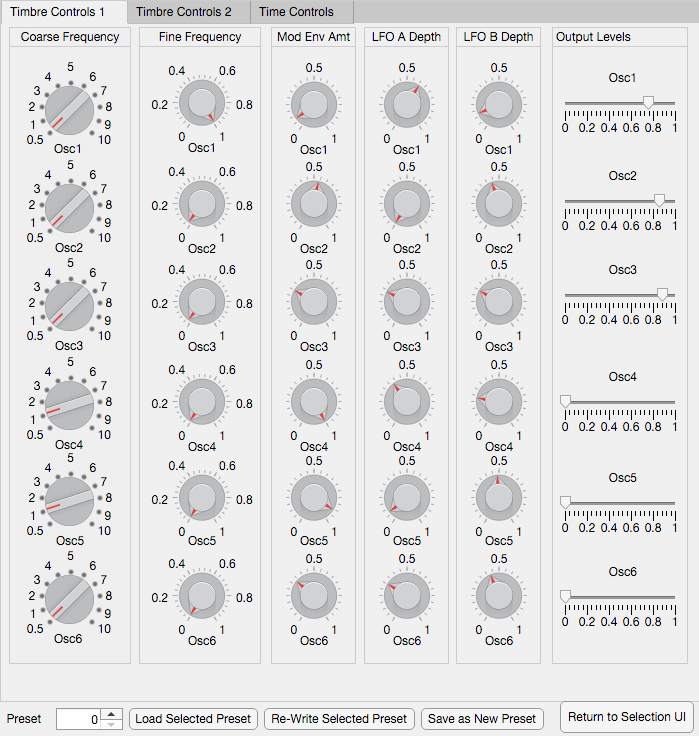
\includegraphics[width = 3in]{TraditionalUI1.png}
\hspace*{0.2cm}
	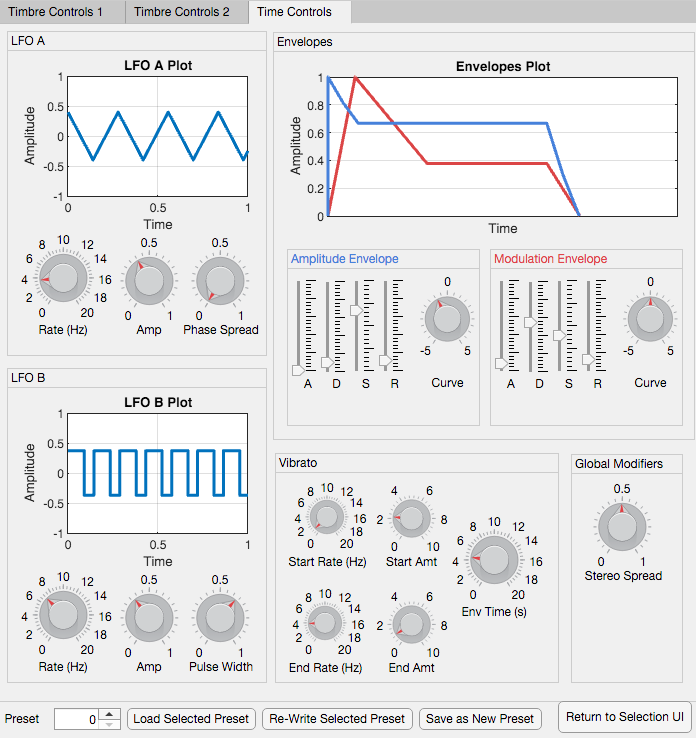
\includegraphics[width = 3in]{TraditionalUI3.png}
	\caption{Traditional Interface - Screen 1 and 3}
	\label{fig:TraditionalInterface}
\end{figure}

\section{Selection Interface}
Typical Soft-Synths are supplied with a large number of presets, which are usually named and arranged into categories. They are usually displayed in a list which can be searched by name, or split into category. In many soft-synths, each preset is given a set (usually 8) of Macro Controls, which each vary single parameter or combinations of parameters, and aim to give the user a quick way to tweak each preset.\\
The Selection Interface is a new approach to displaying presets, arranging the presets as cells of a 2D voronoi diagram, such that similar presets are close to each other and coloured similarly. The presets can quickly be compared by moving the mouse around the diagram, and presets are selected by clicking on the cells. Once a preset is selected it can be edited by macro controls. 
The presets have been divided into a number of categories. Clicking the category buttons at the top of the interface highlights the selected category, as shown in Figure \ref{fig:PCAInterface}. By clicking the 'Display Mode' button, it is also possible to limit the presets displayed to just the selected category(s), displayed in a recalculated voronoi diagram.\\
Both the 2D spacing of the presets, and the creating of the macro controls is calculated automatically from the set of presets' parameter values using Principal Component Analysis (PCA).

\begin{figure}[h] 
	\centering
	\hspace*{-0.2cm}
	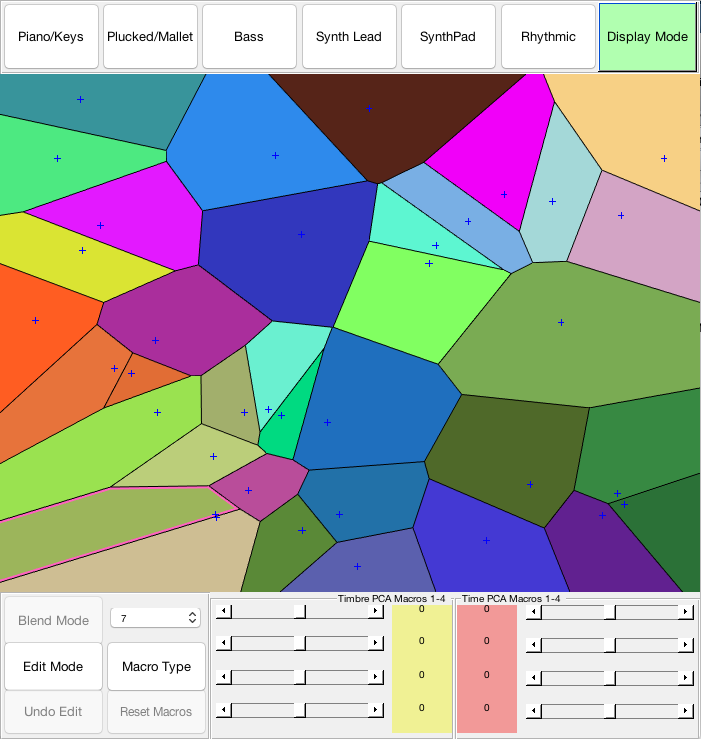
\includegraphics[width = 3.0in]{PCAInterface1.png}
	\hspace*{0.1cm}
	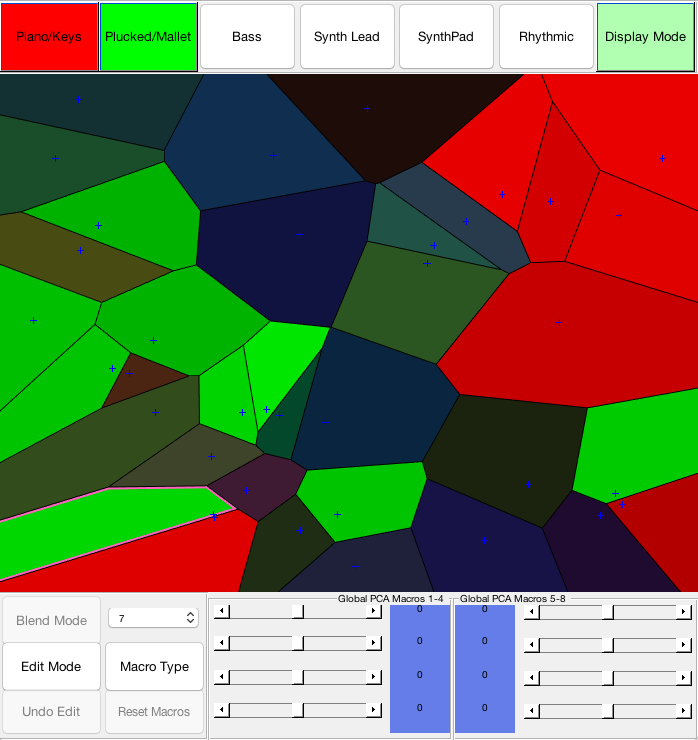
\includegraphics[width = 3.0in]{PCAInterface2.png}
	\caption{PCA Interface - Normal View, and Category Highlight View}
	\label{fig:PCAInterface}
\end{figure}

\section{Blending Interface}
Preset Blending is a somewhat popular approach in synth interface design, where new presets are created by a linear combination of presets. (EXAMPLES: Alchemy, MaxMSP Nodes) The Blending Interface is an extension of this approach.\\
Three initial presets (A, B, C) are selected, and are placed on the corners of the triangle in the centre of the interface. As the cursor moves over the interface, a new preset is created as a weighted sum of the three presets, based on promixity to the corners. Once the user finds the optimal preset in the space, the user clicks. The preset clicked on then becomes the preset A (I.e is placed on the bottom corner of the triangle), and a new preset B and C are generated. \\
This process is repeated as many times as desired, allowing the user to keep searching through the parameter space.\\
If the user clicks on the 'Pause on Selected Preset Button', they are shown an interactive display of their past preset choices, which they can use to go back to previously selected settings and resume searching. It is also possible to select three of the previous presets, and assign them to preset A, B and C.
The user has the option to freeze sections of the parameter space, which helps the search be more fine tuned to their needs.
The colours of the Blending Interface are calculated to be consistent with the Selection Interface.
\begin{figure}[h] 
	\centering
	\hspace*{-0.2cm}
	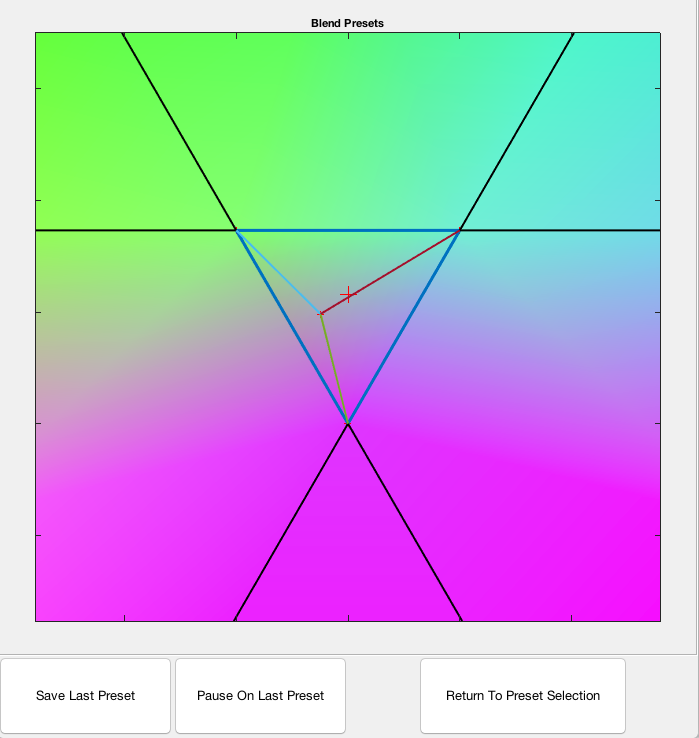
\includegraphics[width = 3.0in]{BlendingInterface1.png}
	\hspace*{0.2cm}
	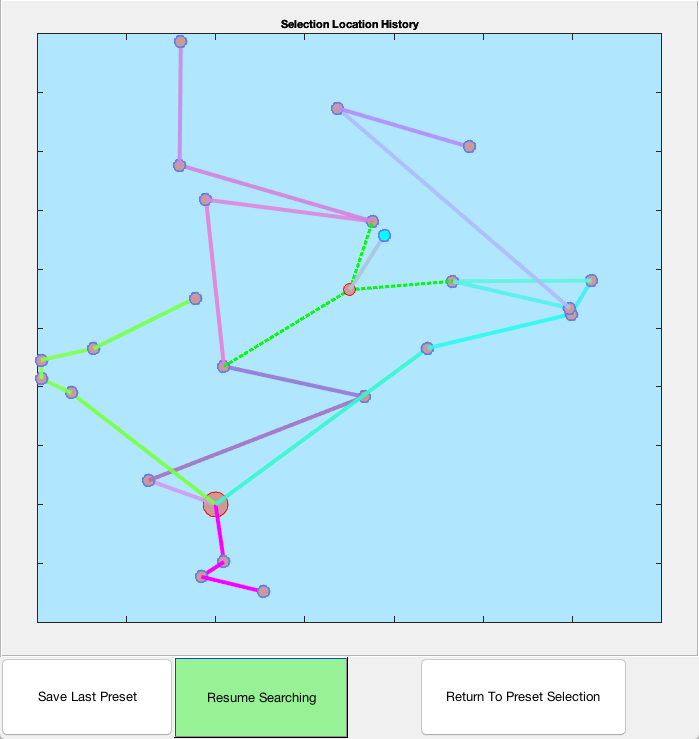
\includegraphics[width = 3.0in]{BlendingInterface2.png}
	\caption{Blending Interface - Normal View, and Selection History View}
	\label{fig:BlendingInterface}
\end{figure}

\section{How the Interfaces are Combined}
When the application is started, the Selection interface is displayed first. Once a preset has been selected and possibly modified with the Macro Controls, the user has the option to click the 'Edit Mode' button, which opens the Traditional Interface, allowing the currently selected preset to be further modified. The user can move back to the Selection Interface by clicking the 'Return to Selection UI' button. The varied preset is displayed on the Selection Interface with a marker, attatched to the original preset, which is positioned and coloured to be consistent with the PCA mapping. If the user wants to undo the edits made to the preset they can click the 'Undo Edit' button. In this way the user can move back and forth between the Blending and PCA interfaces as often as desired.\\
Once three presets have been selected, the user has the option of clicking the 'Blend Mode' button which opens the blending interface, and assigns the three seceted presets to A, B and C. The user can then use the blending interface for as long as necessary, and then click the 'Return to Preset Selection' button. This time another marker is created, with dotted lines to the 3 initially selected presets.\\ 
This marker can then be used in the same way as the cells of the voronoi diagram, I.e it can be previewed by clicking, selected by double clicking, can be edited with the Macro Controls or the Traditional Interface. There are a set of parameter visualisations that are displayed alongside all of the presets to give the user more feedback into what changes they are making, and to aid in understanding how the synthesis algorithm works.
\begin{figure}[h] 
	\centering
	\hspace*{-1.5cm}
	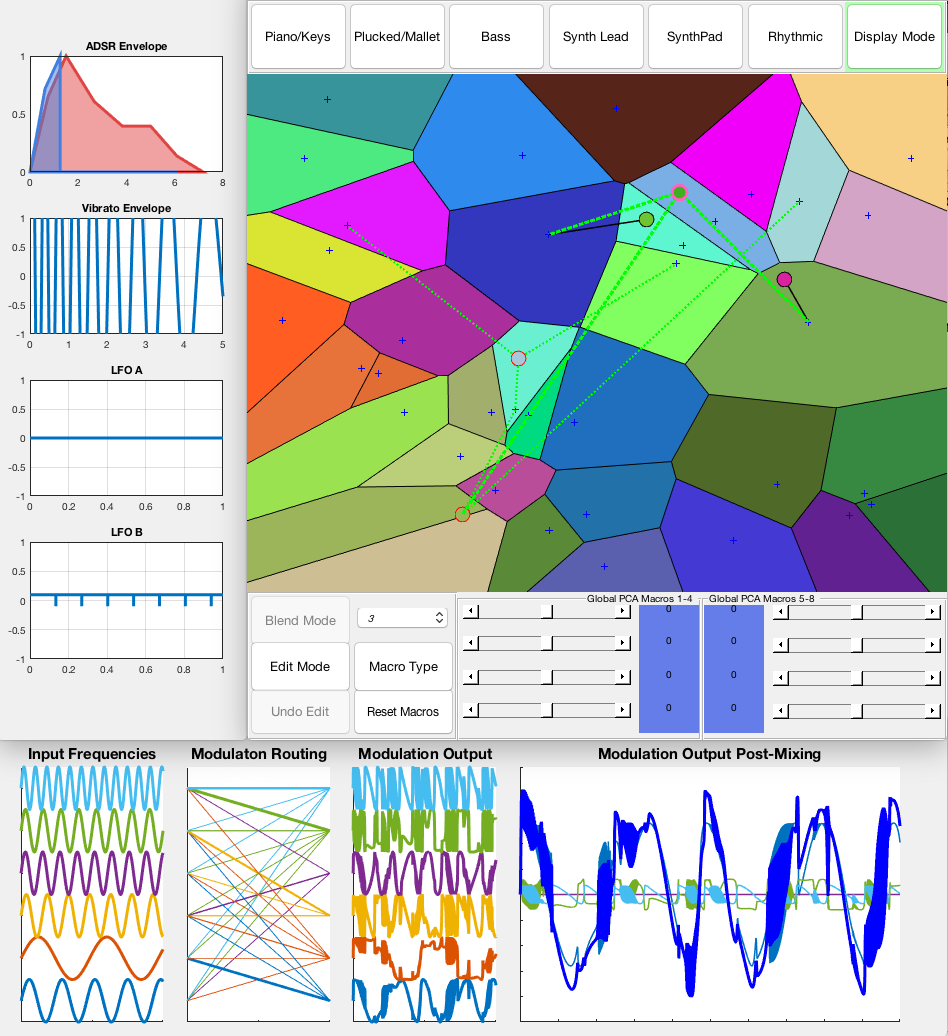
\includegraphics[width = 7.5in]{CombinedInterface1.png}
	\caption{Combined Interface - PCA view}
	\label{fig:CombinedInterface}
\end{figure}

\chapter{Design and Evaluation of Interfaces}
\section{Traditional Interface}
%\subsection{Detailed Description}
\begin{wrapfigure}{r}{0.5\textwidth}
		\vspace{-30pt}
	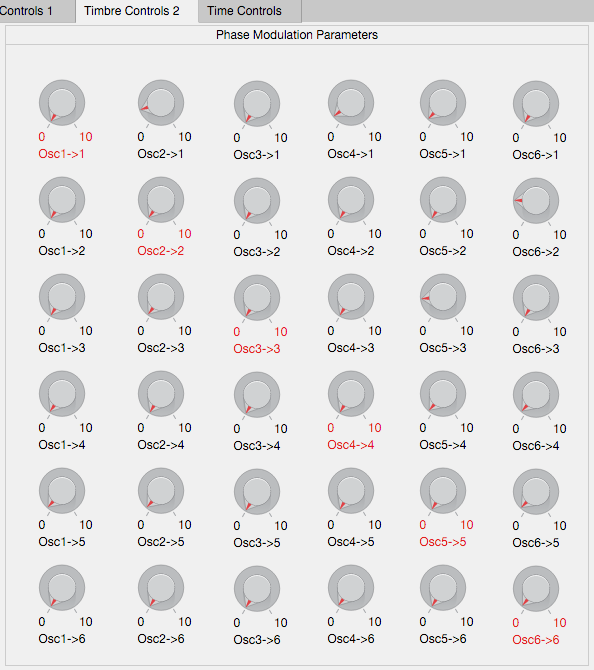
\includegraphics[width = 4in]{TraditionalUI2.png}
	\caption{Traditional Interface - Screen 2}
	\label{fig:TraditionalInterface2}
	\vspace{-60pt}
\end{wrapfigure}
This interface was created in the MATLAB App Designer toolbox. As the parameters are varied, they are sent in real time over OSC to the synthesiser.
\subsection{Strengths}
A skilled user can use knowledge of synthesis to construct any preset they can conceive of. The entire parameter space can be searched. For sectional of the synthesiser archececture that are more intuitive, such as the LFOs and envelopes, this works very well.
\subsection{Weaknesses}
Slow serial control of all of the parameters. Even if the user knows exactly what each parameter should be set to, it will still take several minutes to go through all of the 96 knobs and set them to the correct value. Parts of the synthesis architecture are non-intuitive and fiddly to use, In particular the 36 phase modulation routing parameters shown in Figure \ref{fig:TraditionalInterface2}. If the user doesn't know exactly what they want, or how to acheive a particular sound, this interface can be extremely inefficient and frustrating.

\section{Selection Interface}
%\subsection{Detailed Description}
This interface was created as a Matlab 'figure based application'.
\subsection{Global PCA vs Time/Timbre PCA}
The PCA is calculated in two different ways for different sections of the interface. In 'Global PCA', each of the $36$ presets' $96$ parameters arranged in a $36 * 96$ array. PCA is carried out on this array to produce the Global PCA Weights and Scores. 

In Time/Timbre PCA, the $96$ parameters are partitioned into two sets: $72$ which affect timbre, and $24$ which affect variation of the sound over time (I.e all of the envelope and LFO parameters). PCA is then carried out seperately on the resulting  $36 * 72$, and $36 * 24$ arrays to produce the Time PCA Weights, and the Timbre PCA Weights. 

The Global PCA Weights are used for the XY-RGB mapping of the Voronoi diagram, the Global PCA Macros, and for colouring the Blending Interface. The Time/Timbre PCA Weights are just used for the Time/TImbre Macro Controls.

The user is given the option to switch between the Global, and TIme/Timbre Macro Controls, as the global controls allow a greater ammount to the space to be searched, but the Time/Timbre controls can be more understandable. 
The Macro controls are the same for all presets, but centered on the currently selected preset. I.e. they allow a relative change of parameters not an absolute parameter change.

A possible extension to this approach is to allow parameter freezing, as in the blending interface, and have the PCA Macros automatically be recalculated based on the currently unfrozen parameters.
Another possible extension is to create a unique set of macro controls for each preset, which may make macro controls more useful, but at the sacrifice of consistency between presets.

\subsection{PCA + Histogram Equalisation Description}
When using the Global PCA scores to calculate the XY-RGB position of each preset in the Voronoi diagram, there are some undesirable characteristics of the mapping produced. The sizes of the cells varies dramatically, and the majority of the presets usually get compressed into one of the corners, see Figure \ref{fig:histEqBefore} This is because PCA is linear, and so 'outliers' will skew the diagram, so after rescaling to $[-1, 1]$ to fit in the diagram, the 'inliers' will be compressed to a smaller range'. A similar effect occurs with the colour mapping, causing many of the colours to be similar to each other minimising the dynamic range of the diagram. (MORE DETAIL HERE WITH REFERENCE). In user interface design, users usually associate larger icons with greater importance, therefore it would be preferable for all the presets to be of a similar size, so as not to give uninteded meaning to particular presets.\\
To fix this issue, a variant of an image processing method known as histogram equalisation (REFERENCE) was used, resulting in the mapping shown in Figure \ref{fig:histEqAfter}.

\begin{figure}
	\centering
	\begin{subfigure}[b]{0.45\textwidth}
		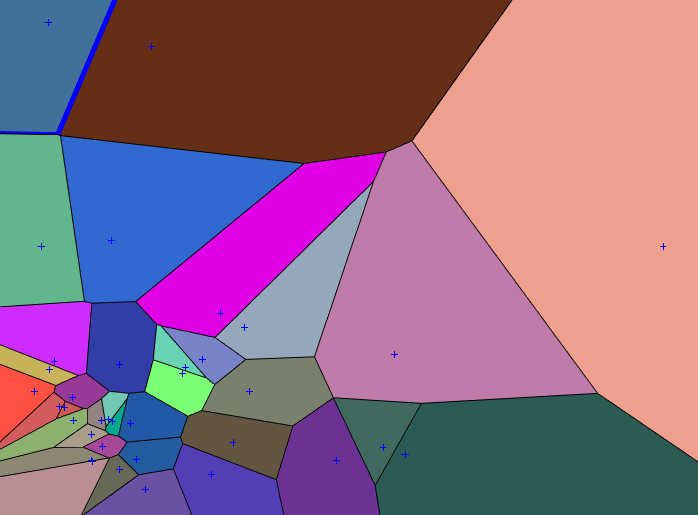
\includegraphics[width=\textwidth]{PCAInterfaceHistEqBefore.png}
		\caption{PCA alone.}
		\label{fig:histEqBefore}
	\end{subfigure}
	~ %add desired spacing between images, e. g. ~, \quad, \qquad, \hfill etc. 
	%(or a blank line to force the subfigure onto a new line)
	\begin{subfigure}[b]{0.45\textwidth}
		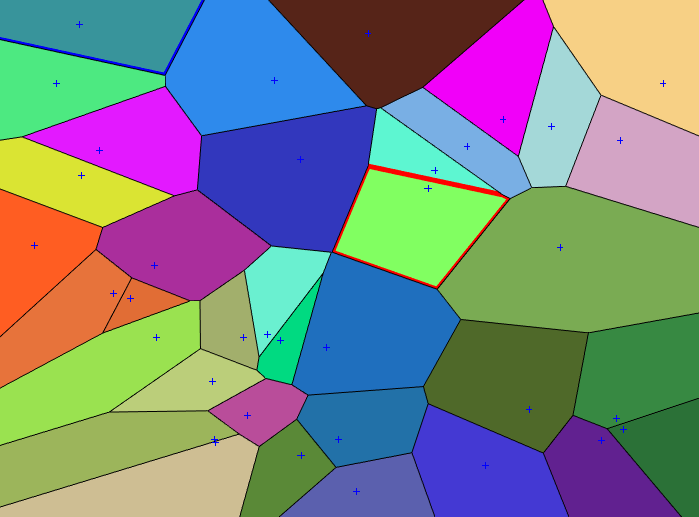
\includegraphics[width=\textwidth]{PCAInterfaceHistEqAfter.png}
		\caption{PCA + Histogram equalisation}
		\label{fig:histEqAfter}
	\end{subfigure}
	\caption{Selection Interface before and after Histogram Equalisation}\label{fig:PCAhistEq}
\end{figure}

The histogram equalisation in one dimension is described in Figure \ref{fig:HistEq}.
\begin{figure}[h] 
	\centering
	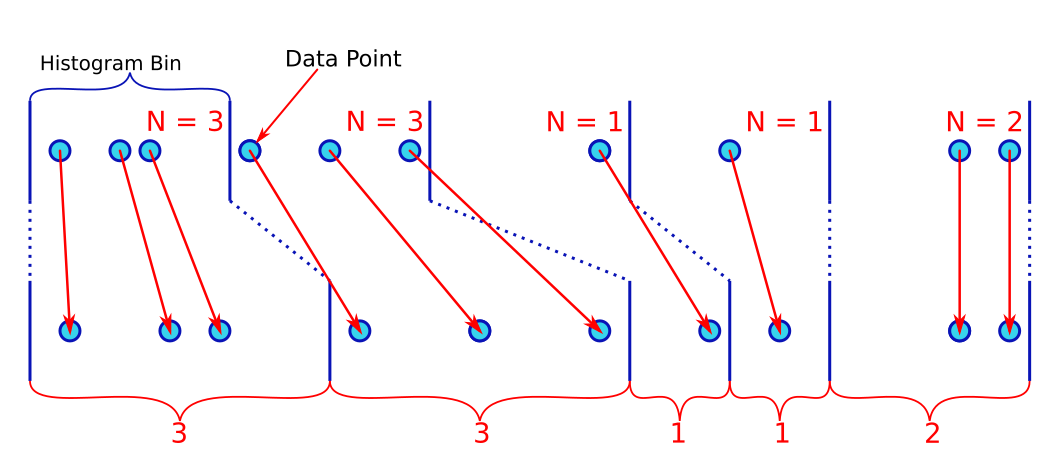
\includegraphics[width = 6in]{HistogramEquilisation.png}
	\caption{Histogram Equalisation}
	\label{fig:HistEq}
\end{figure}
A histogram is created by splitting the data into a number of eqully spaced bins (6 bins was empirically found to work well in this case). The bins are then rescaled, such that the bin width is equal to the number of data points in the bin).

This process is carried out for the presets in all 5 of the XY-RGB dimensions, and then each dimension is mapped to the range $[0.05, 0.95]$, such that it will fit inside the axes of $[0, 1]$. Figures \ref{fig:PCAnumPresets} and \ref{fig:PCAnumPresets2}, show this technique applied to the first 3 principal components.

This approach, although simple, effectively redistributes the presets. As long as one of the bins are empty, the mapping in each dimension is peicewise linear and continuous. This means that the Combined Preset Markers can be positioned correctly on the graph by first calculating the PCA scores, then passing these scores through the mapping function. Due to the continuity of the mapping function, the Macro Controls will cause the preset markers to move smootly across the graph. ... FINISH WRITING
\subsection{Demonstrations of Preset Group Clustering}
Having divided the presets into a set of (non-exlusive) categories, the clustering nature of the PCA process can be tested by viewing where the categories are placed in the diagram, see Figure \ref{fig:Categories}. This demonstrates that the PCA process does indeed cluster the categories together, although some are better clustered than others. Part of this is due to the fact that the categorys are somewhat subjective, for example the decision between Synth Lead and Synth Pad, or between Piano/Keys and Plucked/Mallet.\\
Some of the categories also include a wide range of sounds, especially Rhythmic and Synth Lead, and so have a less consistent pattern in their parameters.
It is also hard to draw colcusions about the clustering performance, due to the small sample size of presets, and the fact that many of the presets were made by using the Blending interface, so potentially have overly similar paramaters than if they'd been made from scratch by a person. To validate this approach more thoroughly, it would need to be applied to many 'real world' sets of presets of pre-existing commercial synthesisers, but several technical challenges (In particular lack of standardisation of control interfaces MORE DETAIL HERE) prevented this being possible during the sort timescale of this project.

\begin{figure}
	\centering
	\begin{subfigure}[b]{0.48\textwidth}
		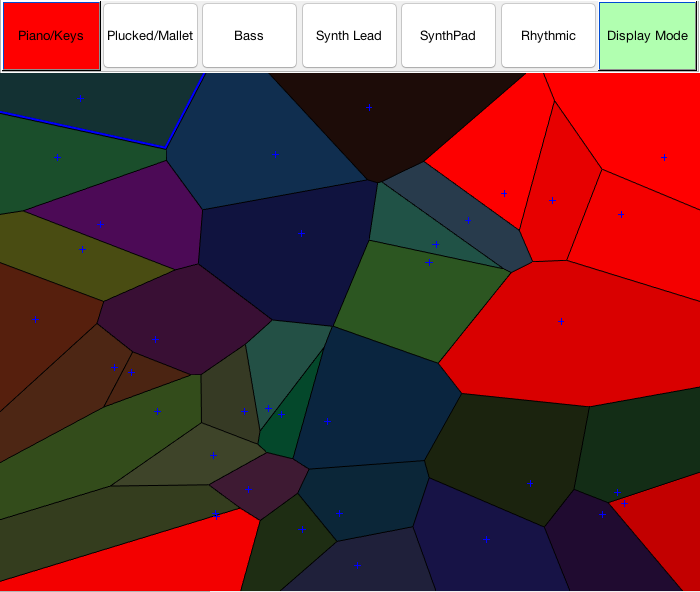
\includegraphics[width=\textwidth]{CategoryPianoKeys.png}
		\caption{Piano/Keys}
		\label{fig:categoriesPianoKeys}
	\end{subfigure}
	~ %add desired spacing between images, e. g. ~, \quad, \qquad, \hfill etc. 
	%(or a blank line to force the subfigure onto a new line)
	\begin{subfigure}[b]{0.48\textwidth}
		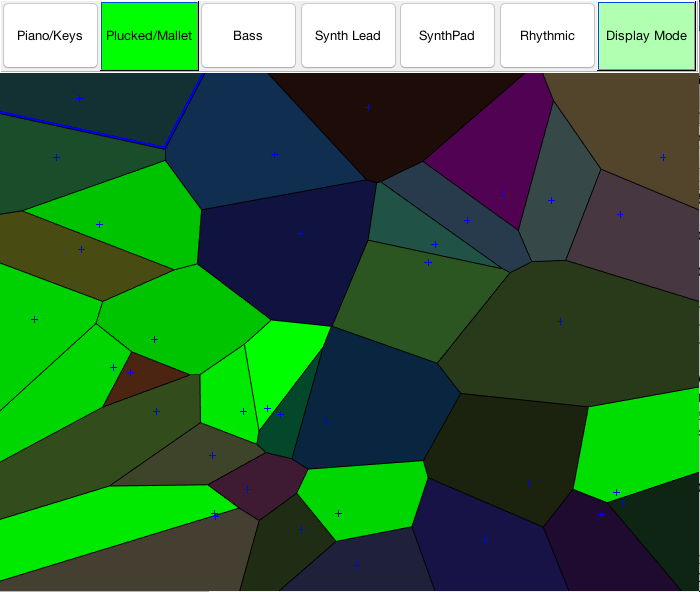
\includegraphics[width=\textwidth]{CategoryPluckedMallet.png}
		\caption{Plucked/Mallet}
		\label{fig:categoriesPluckedMallet}
	\end{subfigure}
\\ 
\begin{subfigure}[b]{0.48\textwidth}
	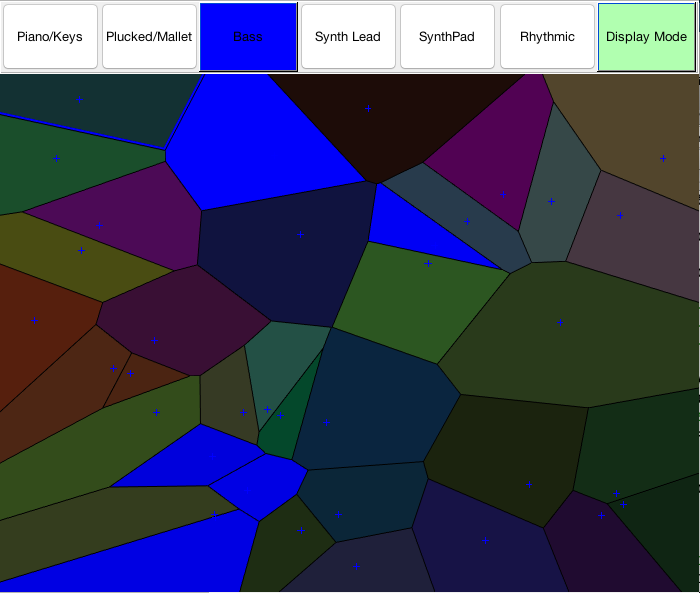
\includegraphics[width=\textwidth]{CategoryBass.png}
	\caption{Bass}
	\label{fig:categoriesBass}
\end{subfigure}
~ %add desired spacing between images, e. g. ~, \quad, \qquad, \hfill etc. 
%(or a blank line to force the subfigure onto a new line)
\begin{subfigure}[b]{0.48\textwidth}
	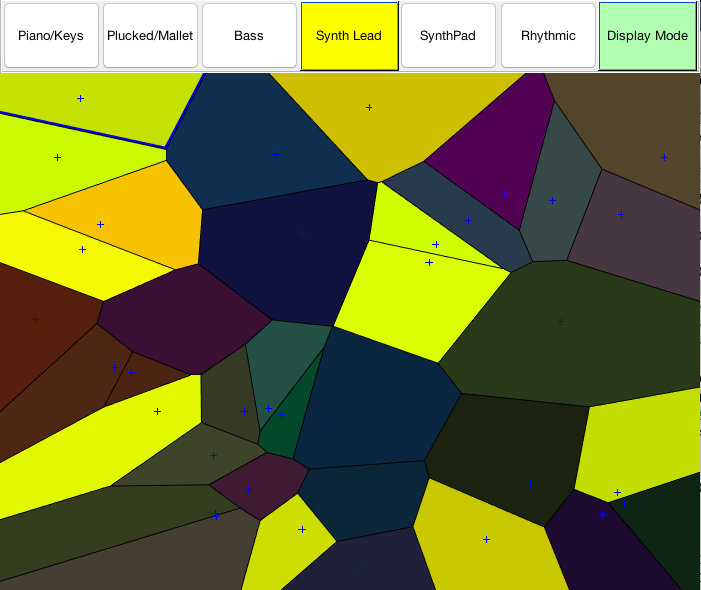
\includegraphics[width=\textwidth]{CategorySynthLead.png}
	\caption{Synth Lead}
	\label{fig:categoriesSynthLead}
\end{subfigure}
\\
\begin{subfigure}[b]{0.48\textwidth}
	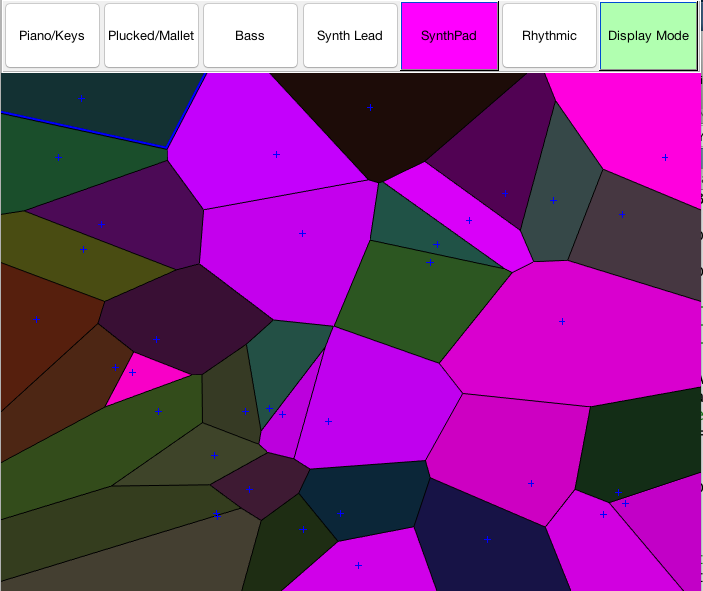
\includegraphics[width=\textwidth]{CategorySynthPad.png}
	\caption{Synth Pad}
	\label{fig:categoriesSynthPad}
\end{subfigure}
~ %add desired spacing between images, e. g. ~, \quad, \qquad, \hfill etc. 
%(or a blank line to force the subfigure onto a new line)
\begin{subfigure}[b]{0.48\textwidth}
	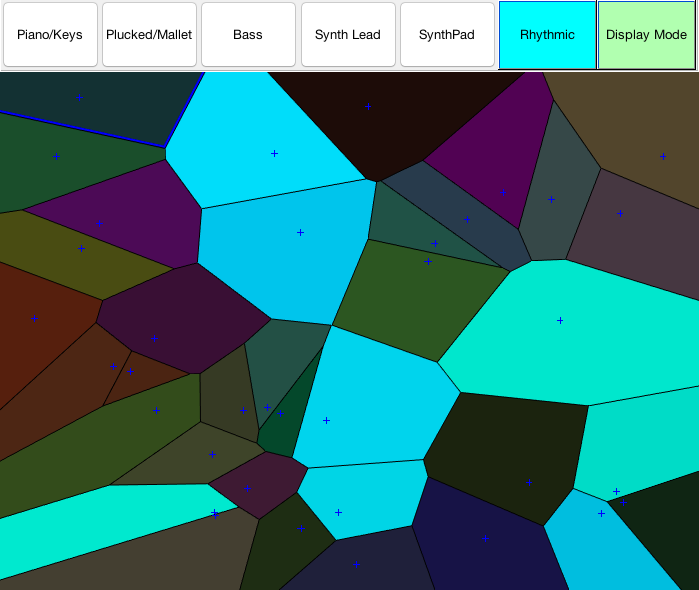
\includegraphics[width=\textwidth]{CategoryRhythmic.png}
	\caption{Rhythmic}
	\label{fig:categoriesRhythmic}
\end{subfigure}
	\caption{Preset Categories shown on Selection Interface}
	\label{fig:Categories}
\end{figure}

\subsection{How the PCA Mapping Scales with Number of Presets}
The consistency of the PCA mapping as more presets are added is of importance to the usefulness of the interface. If the mapping radically changes every time a new preset is added, then any intuitition the user has learned about what the different components represent will be lost. This is one of the reasons for choosing PCA, as the linearity of the technique should lead to less surprising results (EXPLAIN BETTER).\\
Figure \ref{fig:PCAnumPresets} shows the variation of the first two principal components as the presets are added one at a time in the order of creation. After Histogram Equalisation has been applied the components are relatively stable, except at certain points where the component flips sign. These can clearly be seen at preset 34 for $PC_1$, and presets 6, 9, 13, 15, 28, 31:36 for $PC_2$. The bottom row of the figure shows the components after this sign flipping has been corrected by flipping the sign of the component. This makes a dramatic improvement in the stability of the principal components, especially for $PC_2$. This phenomenon also occurs in $PC_{3,4,5}$ used for the RGB mapping of the presets.
\begin{figure}
	\hspace{-80pt}
	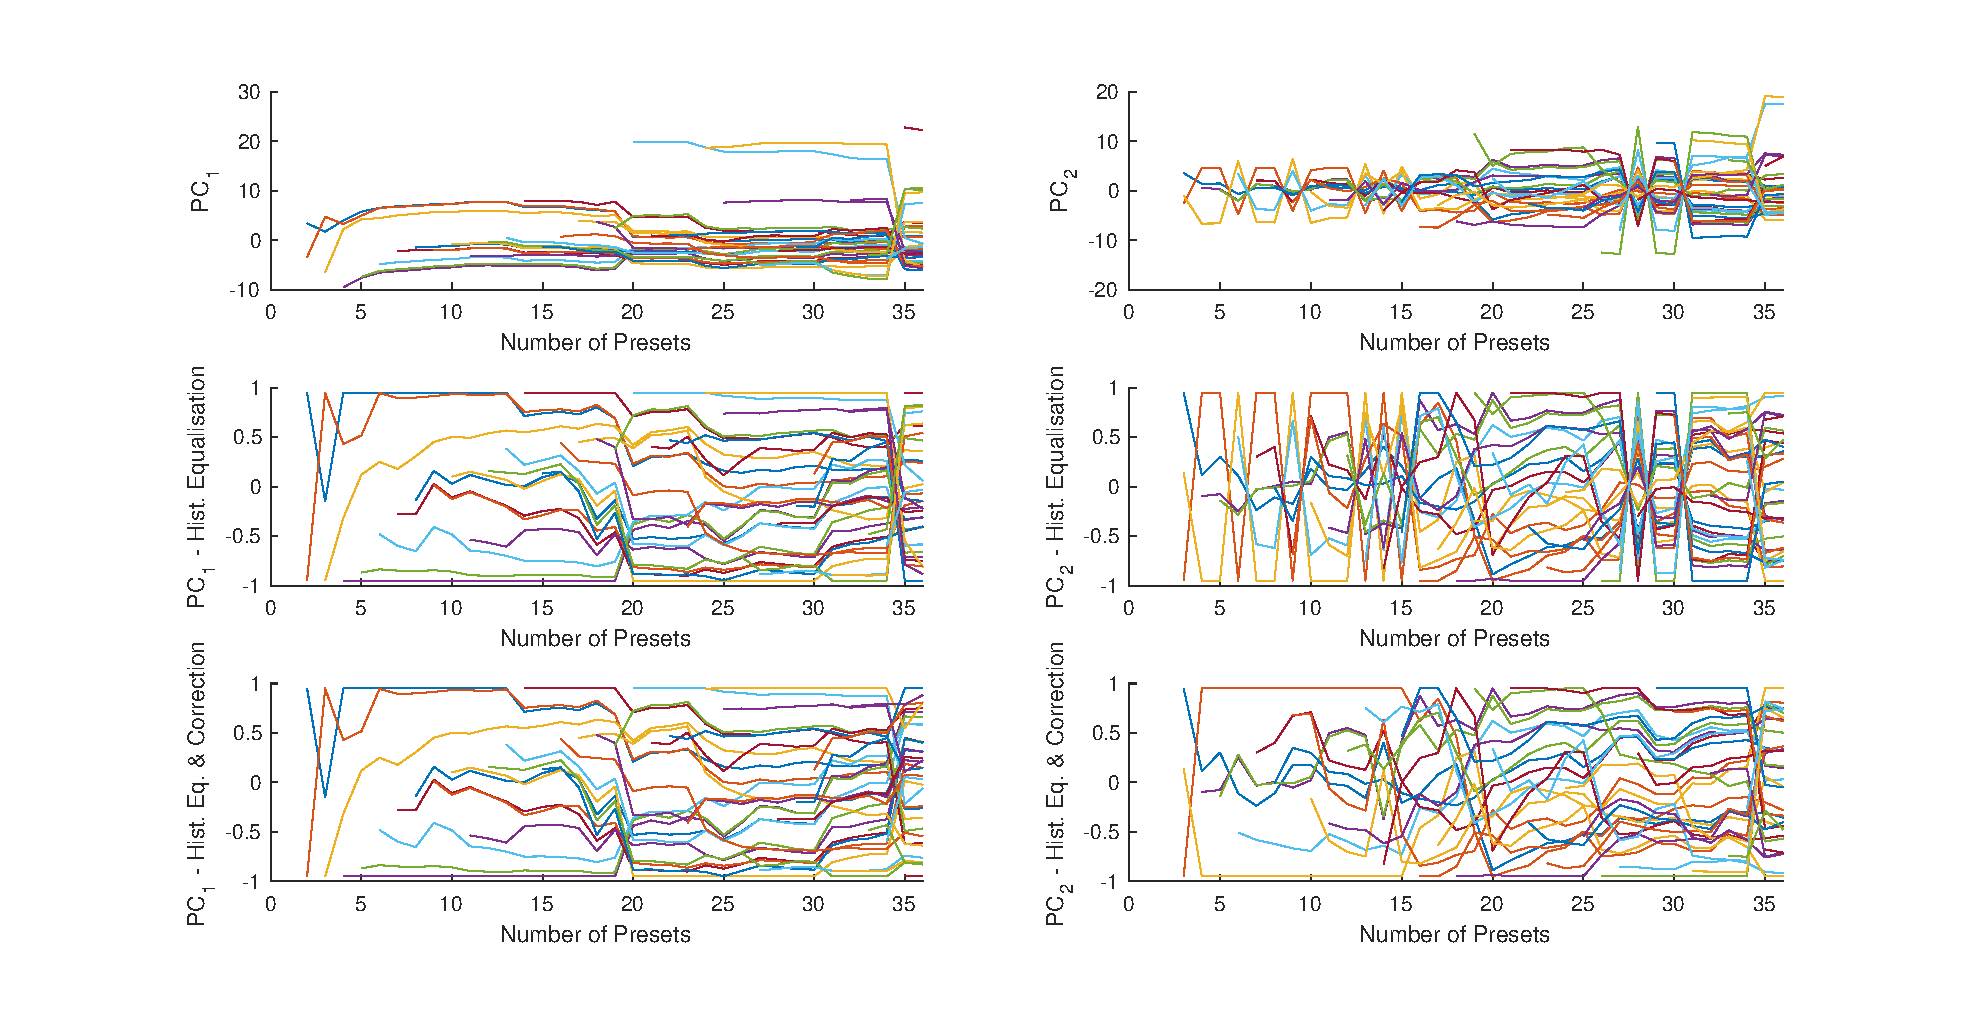
\includegraphics[width = 8.5in]{PCAnumPresets1.eps}
	\caption{PCA stability with number of presets}
	\label{fig:PCAnumPresets}
	%	\vspace{-30pt}
\end{figure}
As PCA is very quick to compute, the necessary sign reversals to correct the components can easily be computed using dynamic programming.\\ Defining $PCA_i^k$ to be the $i$th principal component computed with $k$ presets.
\vspace{-10pt}
\begin{itemize}
		\setlength\itemsep{-1.2em}
	\item 
Iterate from $k = 1$, to $k = N-1$, where $N$ is the number of presets.
	\item 
If $\|PCA_i^{k+1} - PCA_i^k)\|_1 > \|PCA_i^{k+1} - (-PCA_i^k))\|_1$,  flip the sign of all remaining presets.
\end{itemize}
This algorithm is used on $PC_3$ in Figure \ref{fig:PCAnumPresets2}. To implement this checking in the interface, all that it necessary to do is keep track of which components have been flipped, and each time a new preset is added, check if $\|PCA_i^{k+1} - PCA_i^k)\|_1 > \|PCA_i^{k+1} - (-PCA_i^k))\|_1$ to determine whether or not to flip component $i$, and update the record of flipped components.
\begin{figure}
	\hspace{-40pt}
	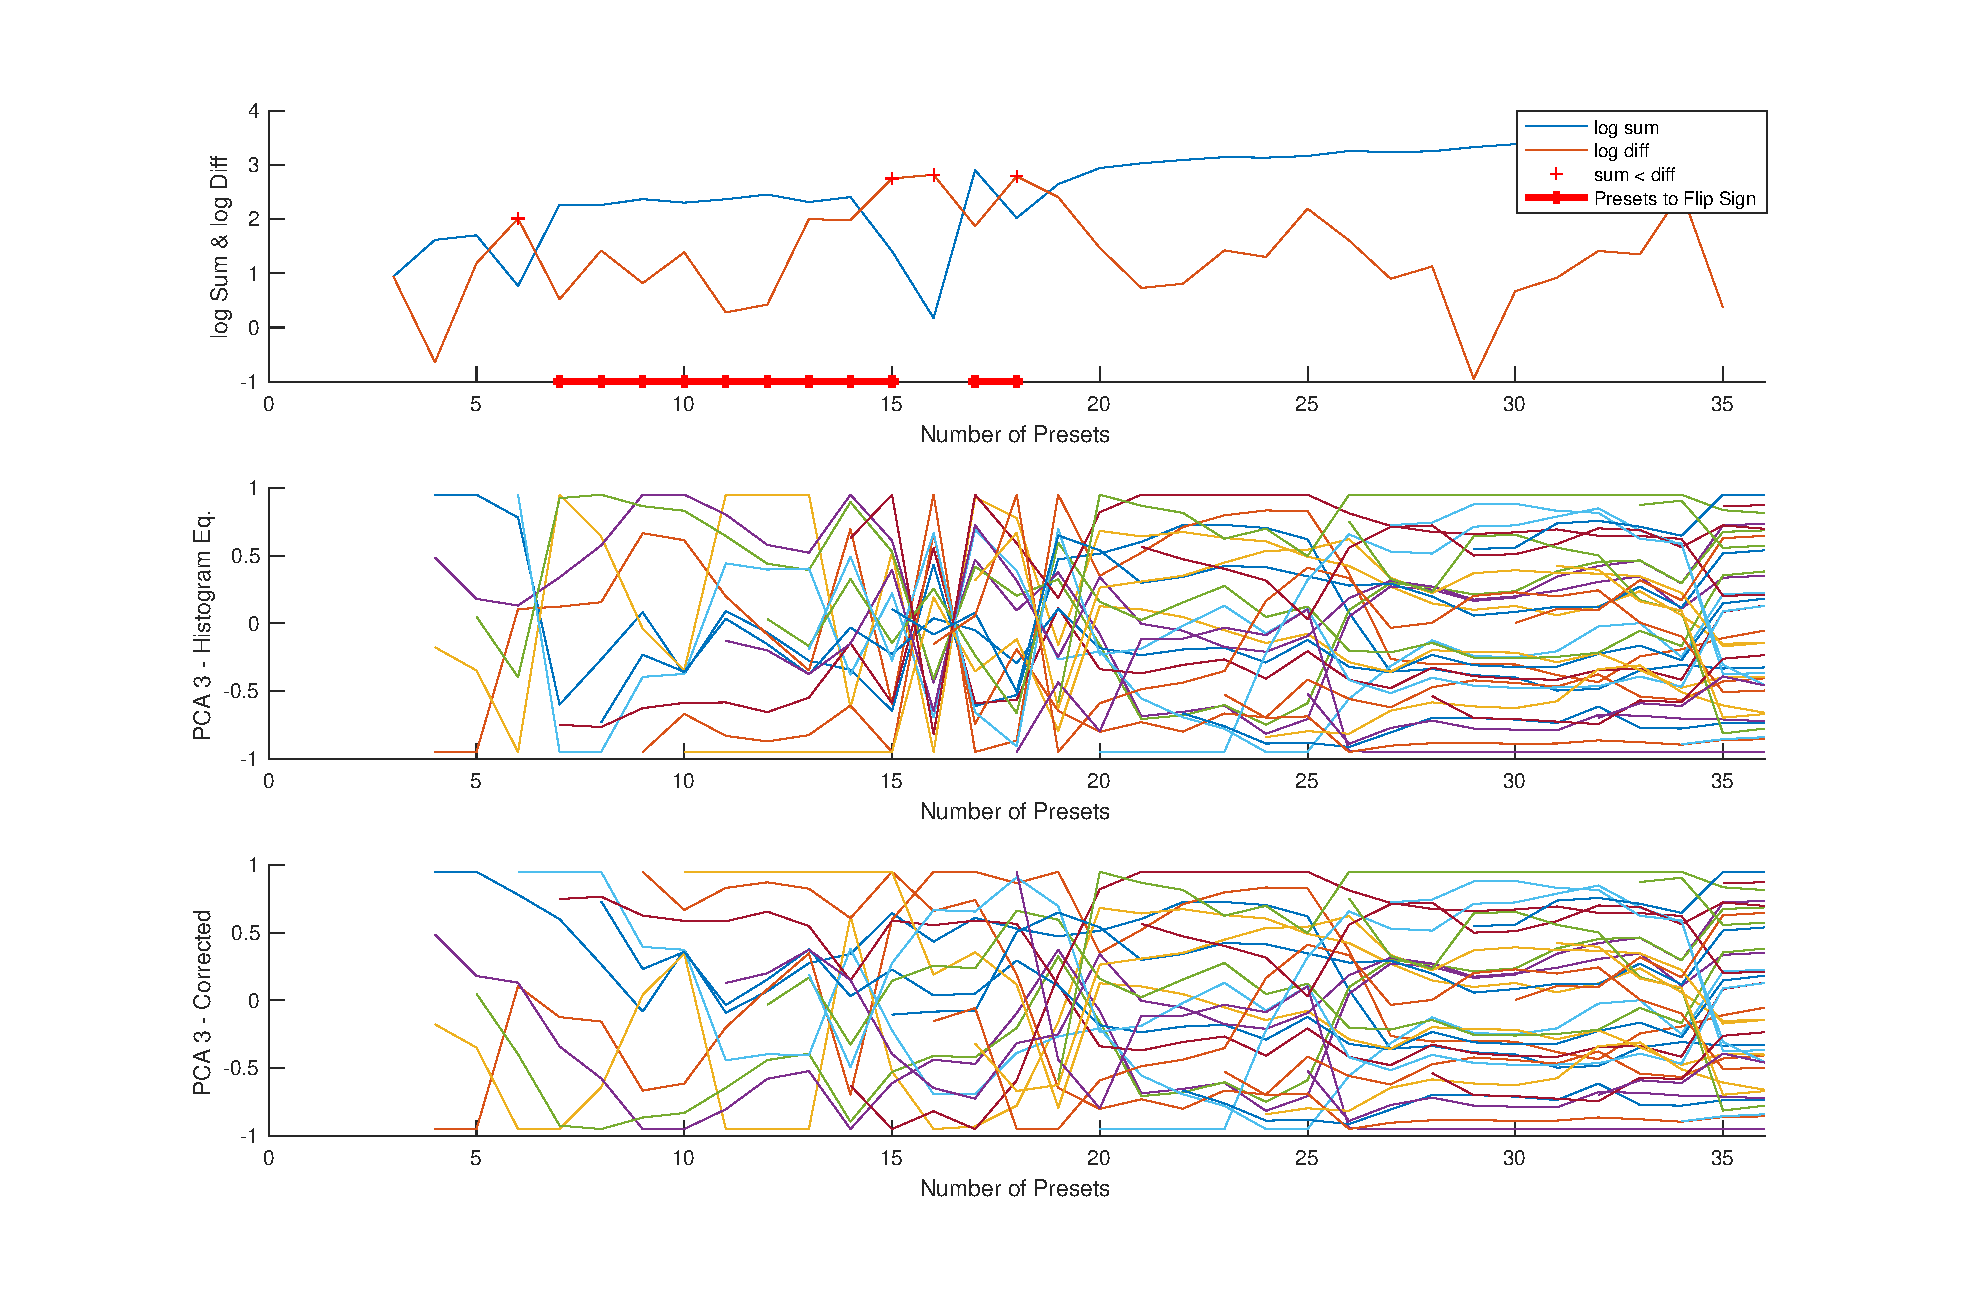
\includegraphics[width = 7in]{PCAnumPresets2.eps}
	\caption{PCA Sign Flip Calculations}
	\label{fig:PCAnumPresets2}
	%	\vspace{-30pt}
\end{figure}

The 'Latent' value for PCA is the variance of each component, and can be used to measure the effectiveness of the PCA mapping. If the first few components account for most of the variance of the dataset, then the dimensionality reduction has been successful.\\
Figure \ref{fig:LatentOriginal} shows how the Latent score changes as more presets are added. Figure \ref{fig:LatentRandom} is the same plot but made with an entirely random dataset of the same size as the original dataset. Comparing the two graphs it can be concluded that the preset dataset is not purely random, as its PCA performs a lot better. Over 50\% of the variance can be accounted for by the first 2 components,  over 90\% can be accounted for by the first 10 components, and the graph seems to have assymtoted to a relatively stable state. In the random dataset, each of the fractions is rougly exponentially decresing as more presets are added. When all 36 random presets are included, only 50\% of the variance can be accounted for by the first 10 components. 

This suggests that PCA is an appropriate technique to use on syntheiser datasets, however testing on more synthesiser datasets is necessary to validate this result.
\begin{figure}
	\hspace{-40pt}
	\begin{subfigure}{3.5in}
		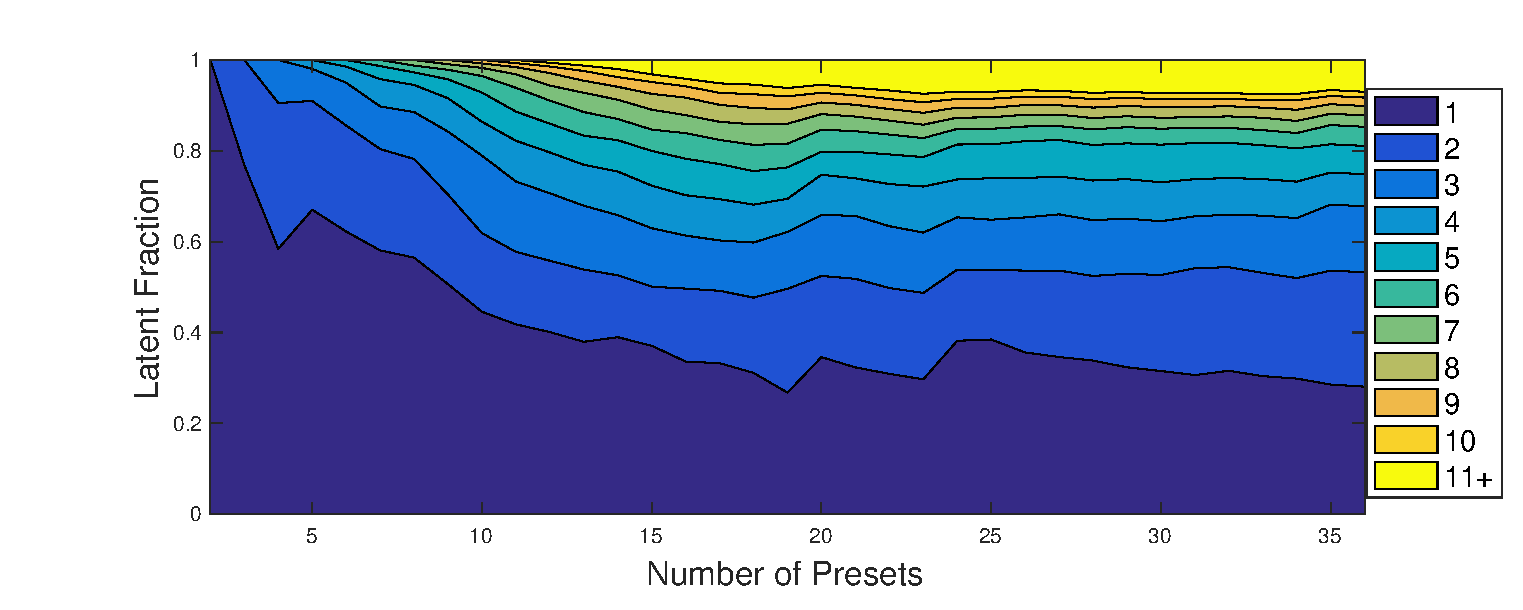
\includegraphics[width = \textwidth]{LatentFraction.eps}
		\caption{Original Presets}
		\label{fig:LatentOriginal}
	\end{subfigure} 
%
	\begin{subfigure}{3.5in}
		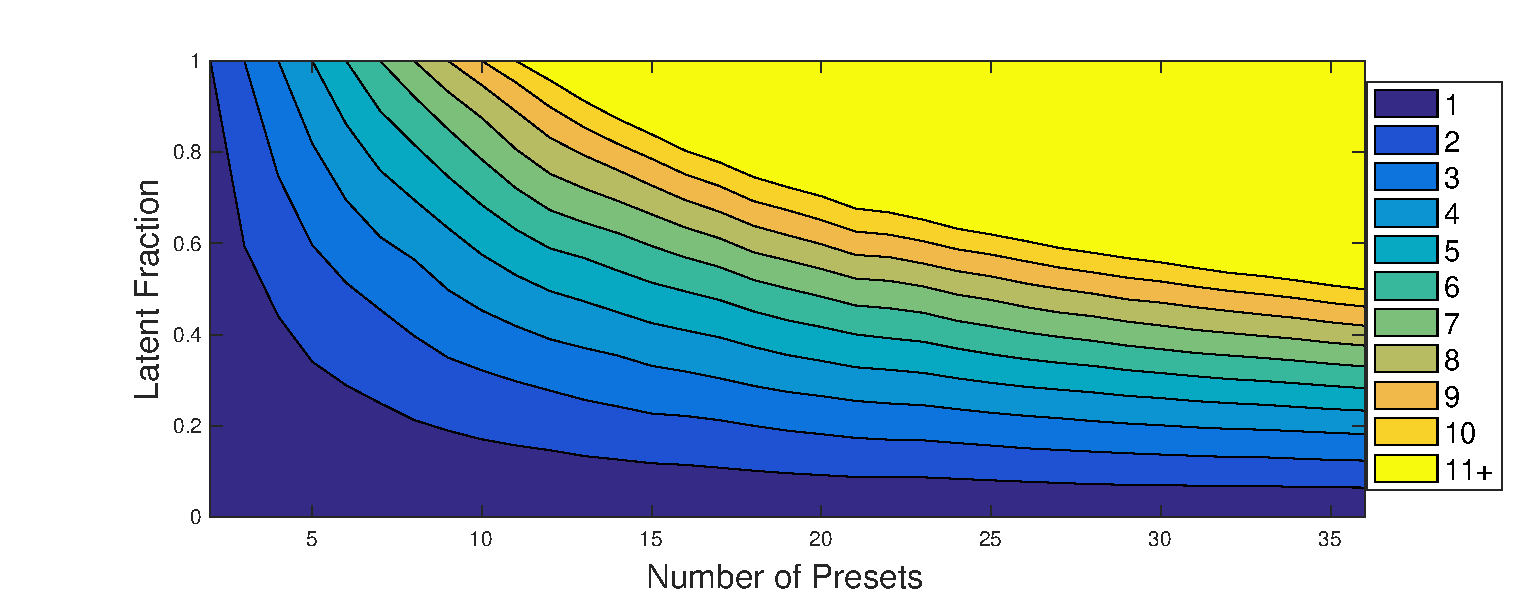
\includegraphics[width = \textwidth]{LatentFractionRandom.eps}
		\caption{Randomised Presets}
		\label{fig:LatentRandom}
	\end{subfigure}
	\caption{Latent Fraction - Colour denotes Principal Component number}
	%	\vspace{-30pt}
\end{figure}


\subsection{Quantify the extra variance the macro controls give}
asdasdasdsa
\subsection{Investigate Permutation Ambiguity}
asdasdsa

\section{Blending Interface}
\subsection{Detailed Description}\label{sec:BlendingDescription}.
This interface was created as a Matlab 'figure based application'.

\begin{figure}[h] 
	\centering
	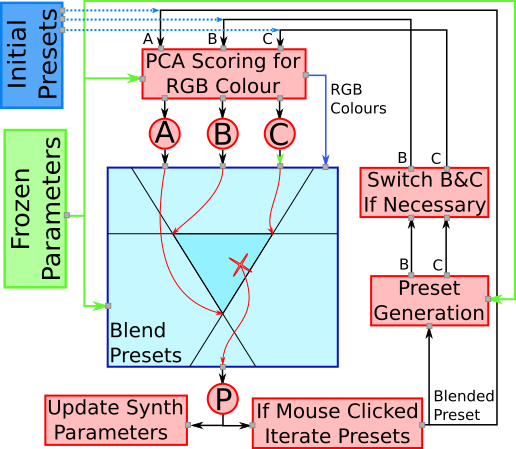
\includegraphics[width = \textwidth]{BlendingAlgorithm.png}
	\caption{Blending Algorithm flow chart}
	\label{fig:BlendingAlgorithm}
\end{figure}

The blending of presets is calculated as a non orthogonal vetor decomposition: (REFERENCE!)
\begin{equation}
	\vec{P} = f(\alpha\vec{A} + \beta\vec{B} + \gamma\vec{C})
	\label{eq:PresetMix}
\end{equation}
Where $\vec{P}$ is the blended preset, $\vec{A}$, $\vec{B}$, $\vec{C}$ are presets A, B and C, $f$ is a function which applies parameter constraints, and $\alpha$, $\beta$ and $\gamma$ are calculated from the following matrix equation:
\begin{equation}
[\beta,  \gamma]^T = (\vec{M}^T*\vec{M})\\vec{M}^T*[x, y], 
	\hspace{1in} \alpha = 1 - (\beta + \gamma)
\end{equation}
\begin{wrapfigure}{R}{0.35\textwidth}
	%\vspace{-30pt}
	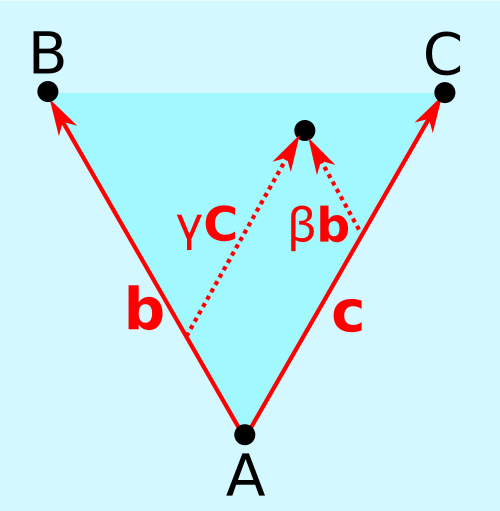
\includegraphics[width = \textwidth/3]{BlendVectors.png}
	\caption{Non-orthogonal vector decomposition}
	\label{fig:BlendingVectors}
	%\vspace{-60pt}
	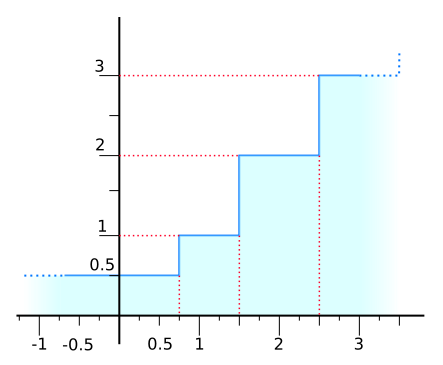
\includegraphics[width = \textwidth/3]{FreqCoarse.png}
	\caption{Mapping from continuous to coarse frequency}
	\label{fig:Freq Coarse}
	%\vspace{-60pt}
	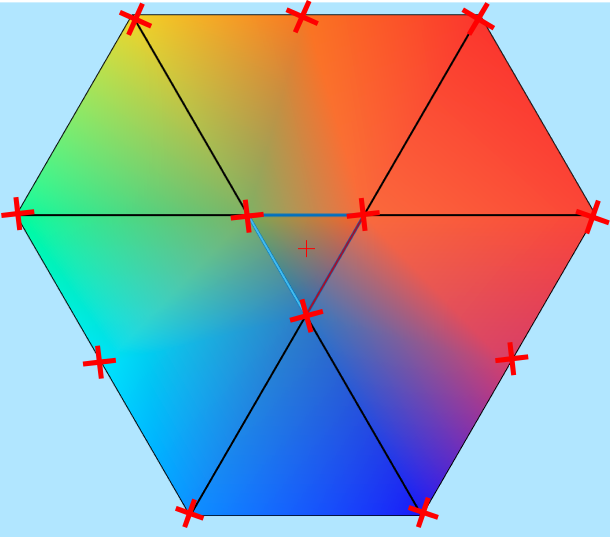
\includegraphics[width = \textwidth/3]{BlendingColours2.png}
	\caption{$PC_{3,4,5}$ applied to RGB colour of blending interface}
	\label{fig:BlendingColours}
	\vspace{-30pt}
\end{wrapfigure}
where $x$, and $y$ are the x and y coordinates of the current cursor position, and $\vec{M} =[\vec{b},  \vec{c}]$, where $\vec{b}$,  $\vec{c}$ are vectors from the A preset location to the B and C preset locations on the interface, as shown in Figure \ref{fig:BlendingVectors}.

The parameter constraint function $f$, applies the relevant constraints to each parameter. Most parameters are continuous with an upper and lower bound, $[l, u]$. For these parameters: $f_i(P_i) = \min(\max(P_i, l), u)$. For the Coarse frequency parameters, the continuous blended value is discretised back into the set ${0.5, 1, 2, 3, ...}$, which the desicion boundary between neighbouring number falling equidistant to the numbers, as shown in Figure \ref{fig:Freq Coarse}.

To make the iterative blending process more intuitive, and to maintain consistency between the interfaces, the RGB colouring using PCA from the Selection interface was used. This is done by using Equation \ref{eq:PresetMix} to calculate the blended preset at each of the points marked on Figure \ref{fig:BlendingColours}, then calculateing the PCA Scores for each of these points. $PC_{3,4,5}$ are mapped to RGB colour, and colour is linearly interpolated between the points. A more detailed colour space could be acheived by using more points, but there would be an associated performance tradeoff. 

Each time the presets are iterated, and a new B and C are generated, the first principal component, $PC_{1}$ is calculated for B and C, and if $PC_{1}^B > PC_{1}^C $, then presets B and C are swapped. The effect of this is that the $x$ direction in the Blending Interface corresponds to a direction of increasing $PC_{1}$. This is done because $PC_{1}$ is also used in the Selection Interface for the $x$ coordinate of each preset, and so this process further maintains consistency between the two interfaces.

\begin{wrapfigure}{R}{0.3\textwidth}
	\centering
	\vspace{-40pt}
	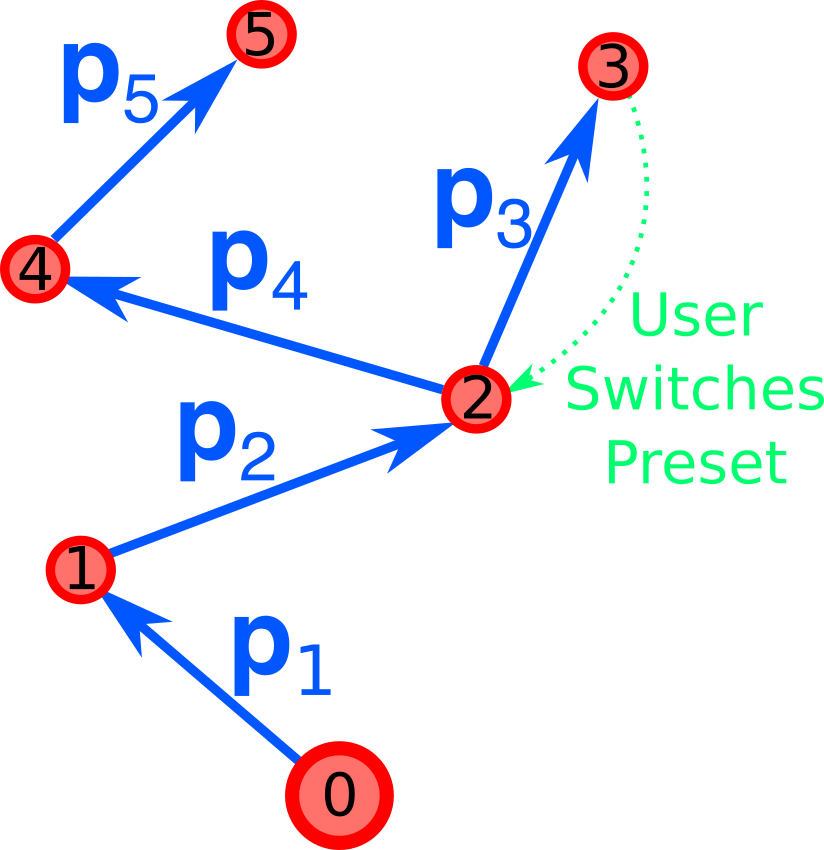
\includegraphics[width = \textwidth/3]{SelectionHistory.png}
	\caption{Selection History plot construction}
	\label{fig:SelectionHistory}
	
	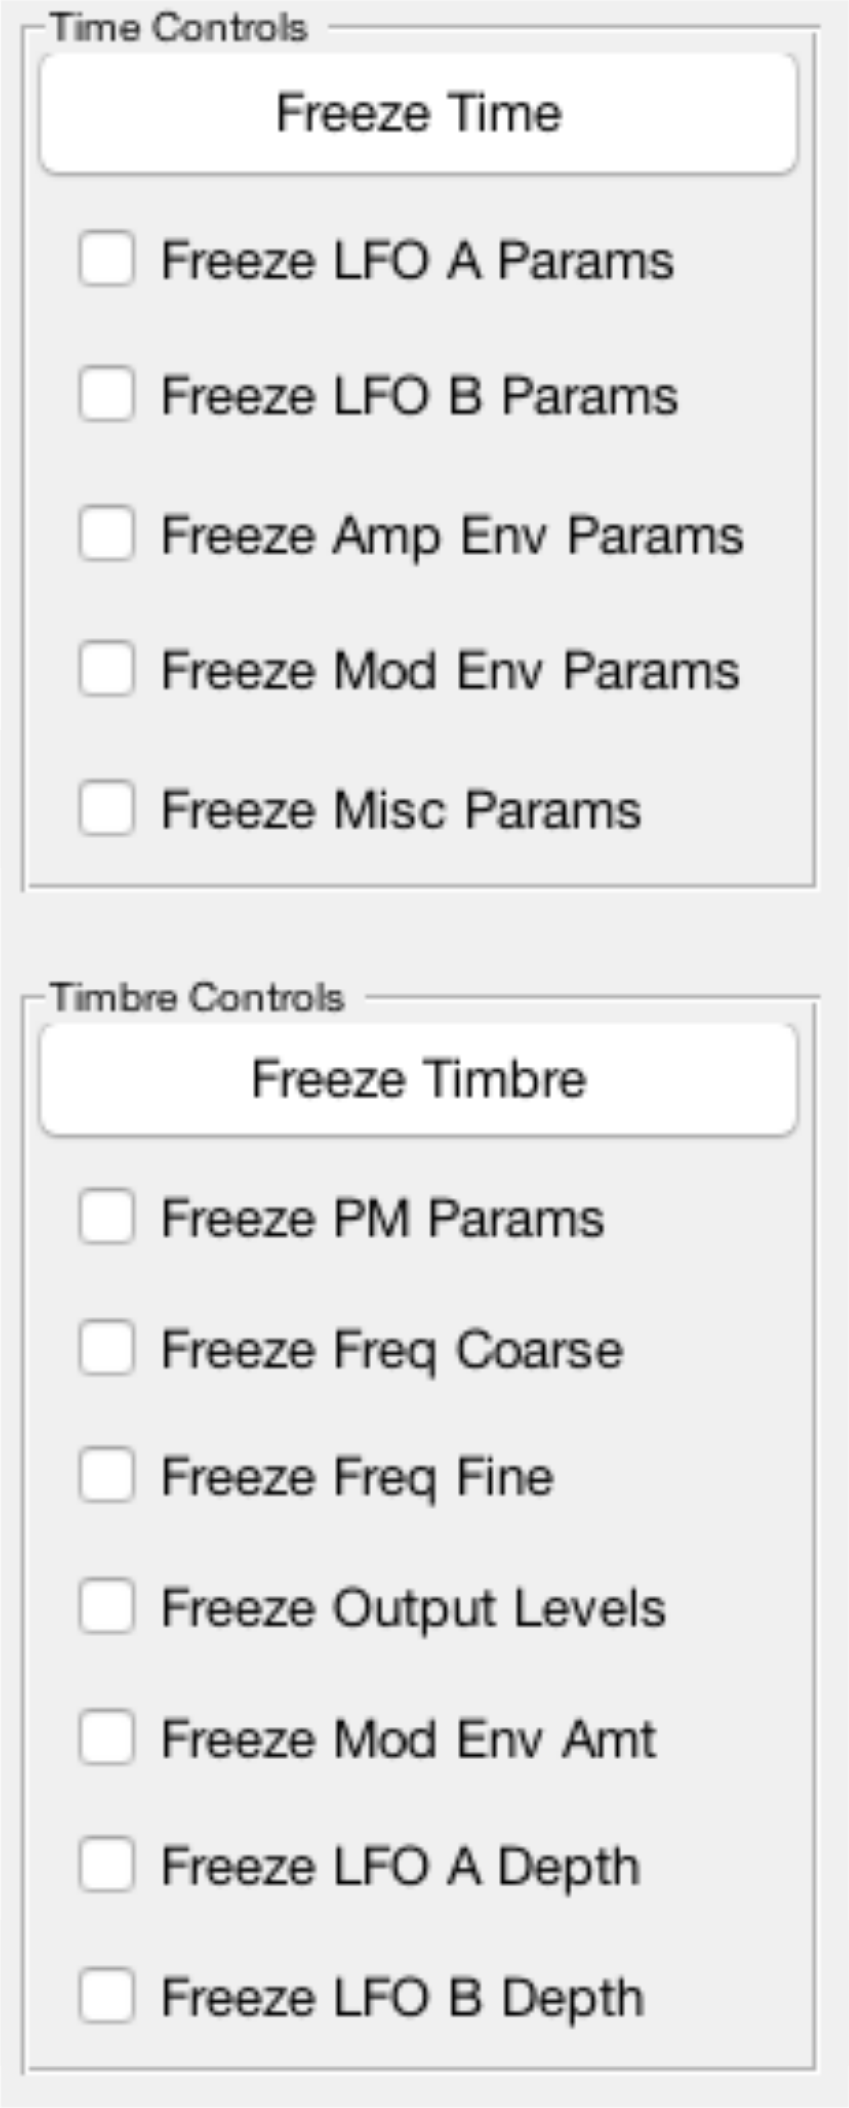
\includegraphics[width = \textwidth/3]{FreezeParams2.png}
	\caption{Parameter Freezing}
	\label{fig:FreezeParams}
	
	\vspace{-30pt}
	
\end{wrapfigure}
The Selection History display, allows the user to browse their previously selected presets, by clicking on nodes of the graph. Each time presets are iterated, the vector from A to the selelected coordinates, $\vec{p}_i$ is recorded. The graph is constucted by joining these vectors head-to-tail, as shown in Figure \ref{fig:SelectionHistory}. The colours of each edge of the graph are chosen based on $PC_{3,4,5}$ of the presets. See Figure, \ref{fig:BlendingInterface} for a typical example of the Selection History plot.

It may be possible to use some of the information contained in the graph (if the data from many users is collected), as a way to refine the preset generation algorithm. If the generation algorithm is producing good presets, then most of the choices should be somewhere between A, B and C on the interface. If the algorithm is producing bad presets, most of the choices will be very close to, or below A. MORE DETAIL HERE

As part of the blending interface, the user has the option to freeze sections of the parameter space. The parameters are divided into 'Time' and 'Timbre' parameters, and then subdivided into a total of 12 smaller categories, see Figure \ref{fig:FreezeParams}. This makes the blending interface more useful, as it allows users with knowledge of synthesisers to fine-tune the blending process to their needs. This tends to lead to more useful generated presets, as it reduces the dimensionality of the search space (BACK THIS UP).

\subsection{Development / Verification of Preset Generation Algorithm using Image Editing Interface}
asdasdsadsa
\subsubsection{Tests of Image Comparison Metric}
asdasdasd
\subsubsection{Convergence Tests for different preset generation algorithms}
asdasdasd
\subsection{Investigate Permutation Ambiguity}
asdasdsad

\chapter{Numerical Comparisons of Interfaces}
Due to the subjectivity of interface design, and as the three interfaces have quite different purposes, there are not many obvious metrics to use to compare the interfaces with each other. However, the key challenge is to make the combined interface better than the traditional interface alone. MORE WRITING
\section{Perfect /Imperfect User Model}
A way of evaluating the performance of the interface is to simulate a 'Perfect User', and an 'Imperfect User' carying out particular tasks. In particular the task is to use the interface to move from an initial preset, to a goal preset. This analysis won't account for any creativity based goals of the interface, but will help evaluate some of the practical comsiderations of the interface. (BAD WORDING< WORK ON THIS SECTION).
 
The Perfect User has perfect knowledge of the synth and the interface, so can always choose the optimum position for a particular knob, or choose the optimum blend of presets in the Blending Interface.

The Imperfect User has imperfect knowledge of the synth and the interface, so chooses interactions similarly to the Perfect User, but 'misses' by a certain ammount: $\Delta P_i = \Delta P_i^0 * (1 + \varepsilon)$, where $\Delta P_i^0$ is the Perfect parameter change, and $\varepsilon$ is a zero mean gaussian random variable with variance $\sigma^2$. Various values of $\sigma$ will be considered to account for the varying skill levels of users.

A key consideration for the Traditional Interface is the order which parameters are varied. In the 'Perfect Order', parameters are visited in decreasing order of importance. In the 'Random Order', parameters are visited in a comploetely random order. Real users most likely operate somewhere in the middle of these regimes. (REFERENCE FOR THIS>???)

\section{Error Metric}
A parameter based error metric is used for these tasks due to the complexity of using a sound based error metric (AS DESCRIBED IN SECTION). 

For each parameter, $p_i$, a weighted $L_1$ norm is used. The parameters are weighted based on an approximate measure of importance, and normalised by their parameter ranges. The total error is calculated as:
\begin{equation}
E = \sum_{i=1}^{N} \| p_i - p_i^{goal} \|_1 *\frac{w_i}{r_i}
\end{equation}
where $w_i$ is the scalar importance weighting for the $i$th parameter, and $r_i$ is the range of values that parameter $i$ can take, see Table \ref{tab:Params}.

The $L_1$ norm was chosen over the $L_2$ norm so that a few large parameter errors don't dominate the error metric and as no gradients are necessary.
This is by no means a perfect metric for comparins synth settings, but it is good enough for our purposes. (IS IT?)
%COULD USE THE Index of Search Space Reduction (ISSR) Approach from Robert Tubbs thesis.
\section{Comparison of isolated interfaces}
\subsection{Traditional Interface}
\begin{wrapfigure}{r}{0.5\textwidth}
	\centering
	\vspace{-60pt}
	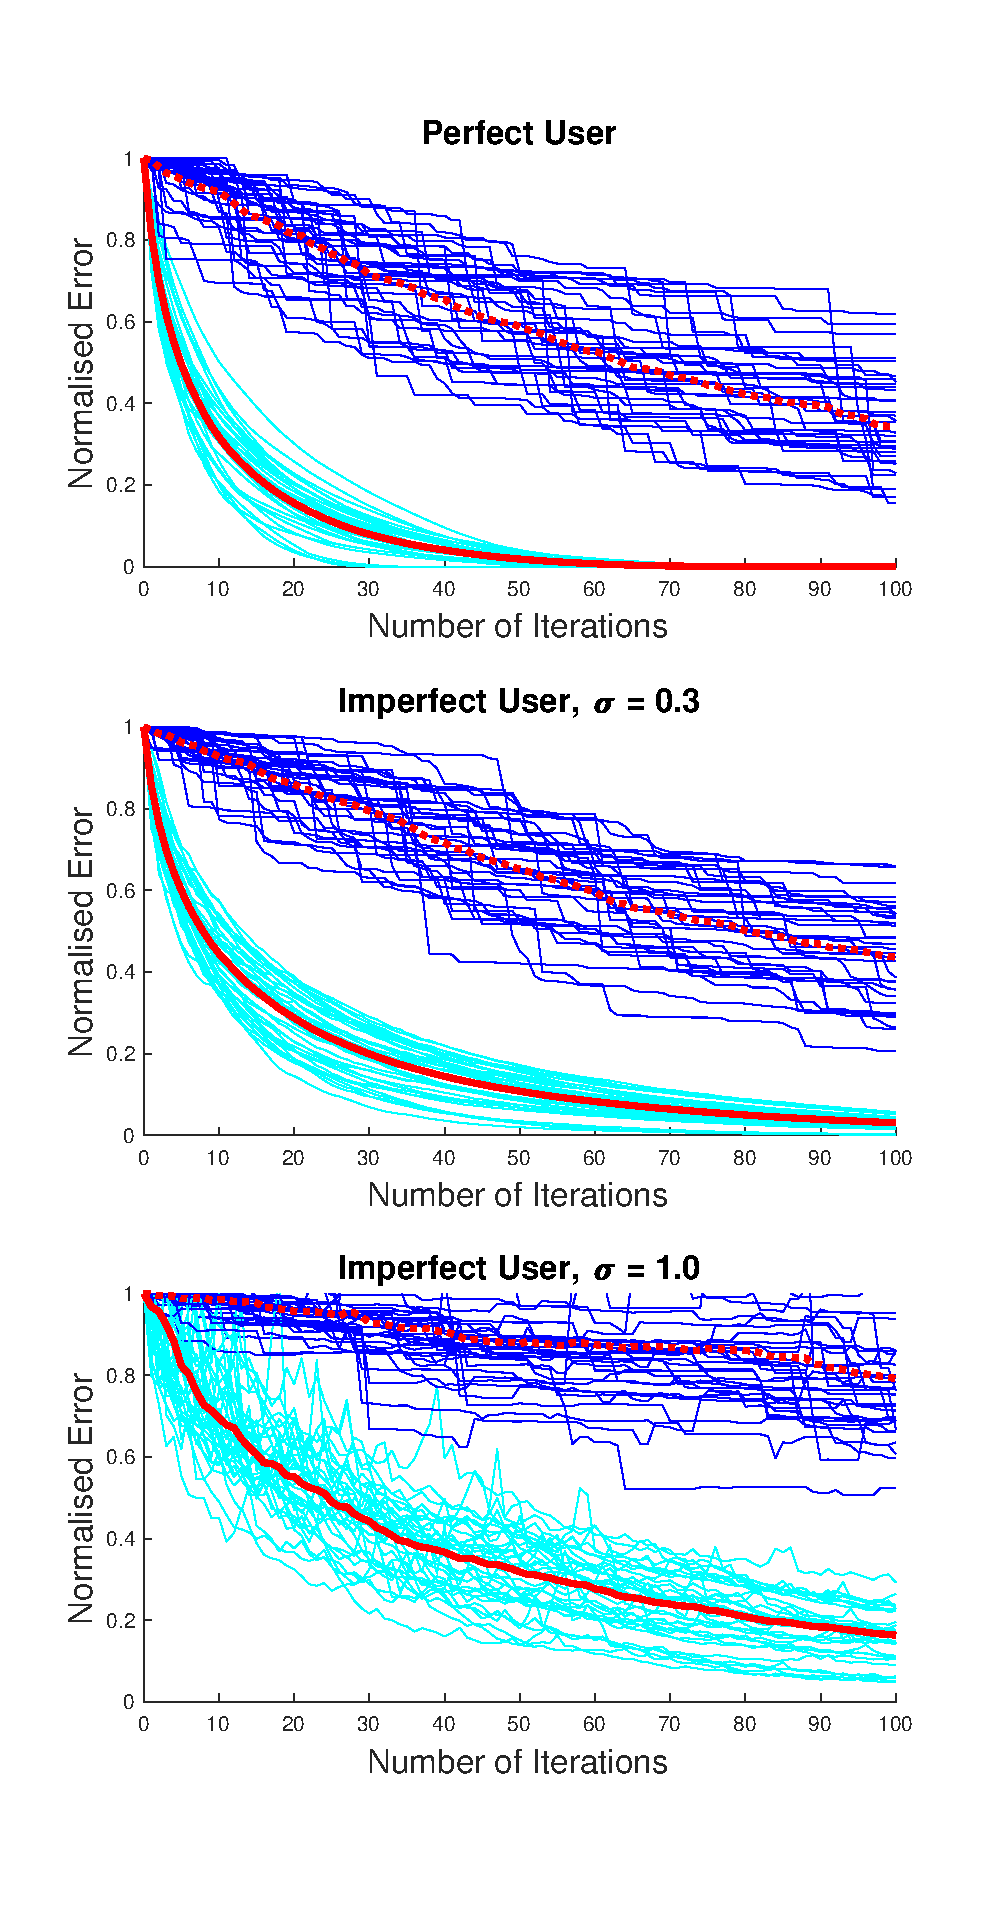
\includegraphics[width = \textwidth/2]{TradInterfaceTests1.eps}
	\caption{Perfect/Imperfect user tests for Traditional Interface}
	\label{fig:TradTest1}
	
%	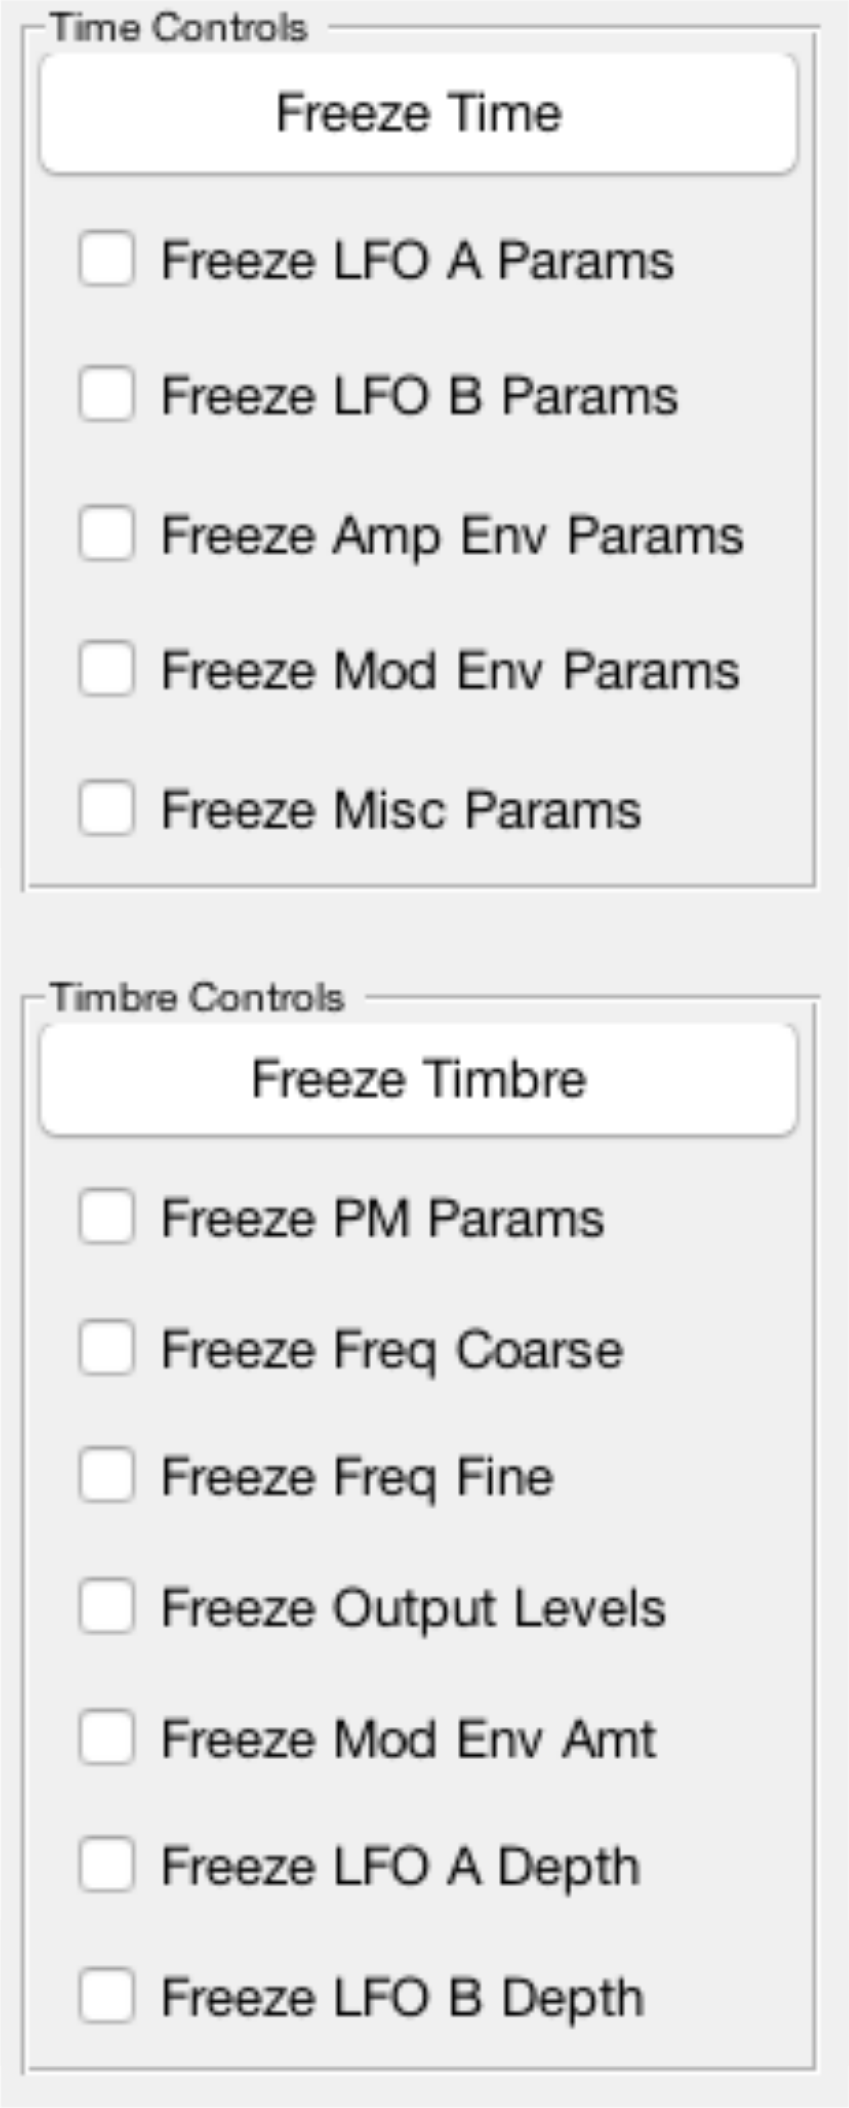
\includegraphics[width = \textwidth/3]{FreezeParams2.png}
%	\caption{Parameter Freezing}
%	\label{fig:FreezeParams}
	
	\vspace{-140pt}
	
\end{wrapfigure}
Perfect/Imperfect user tests were carrried out on the blending interface, using each of the 36 presets as a goal preset, and setting the starting preset to the closest preset to the goal preset. The results of these tests are shown in Figure \ref{fig:TradTest1}. In each of the plots, the cyan lines are individual instances of the Perfect Order test. The blue lines are individual instances of the Random Order test. The solid red line is the mean of the Perfect Order tests, and the red dotted line is the mean of the Random Order tests. 

For low values of $\sigma$, the Perfect Order tests folllows a smooth, approximately exponentially decreasing, curve. For high values of $\sigma$, and when the random otder is used, the error decreases in a much less smooth manner. In all cases the Perfect Order gives a substantially faster convergence time. A comparison of the mean error for various values of $\sigma$ is shown in Figure \ref{fig:TradTest2}. 
\begin{figure}
	\centering
%	\vspace{-40pt}
	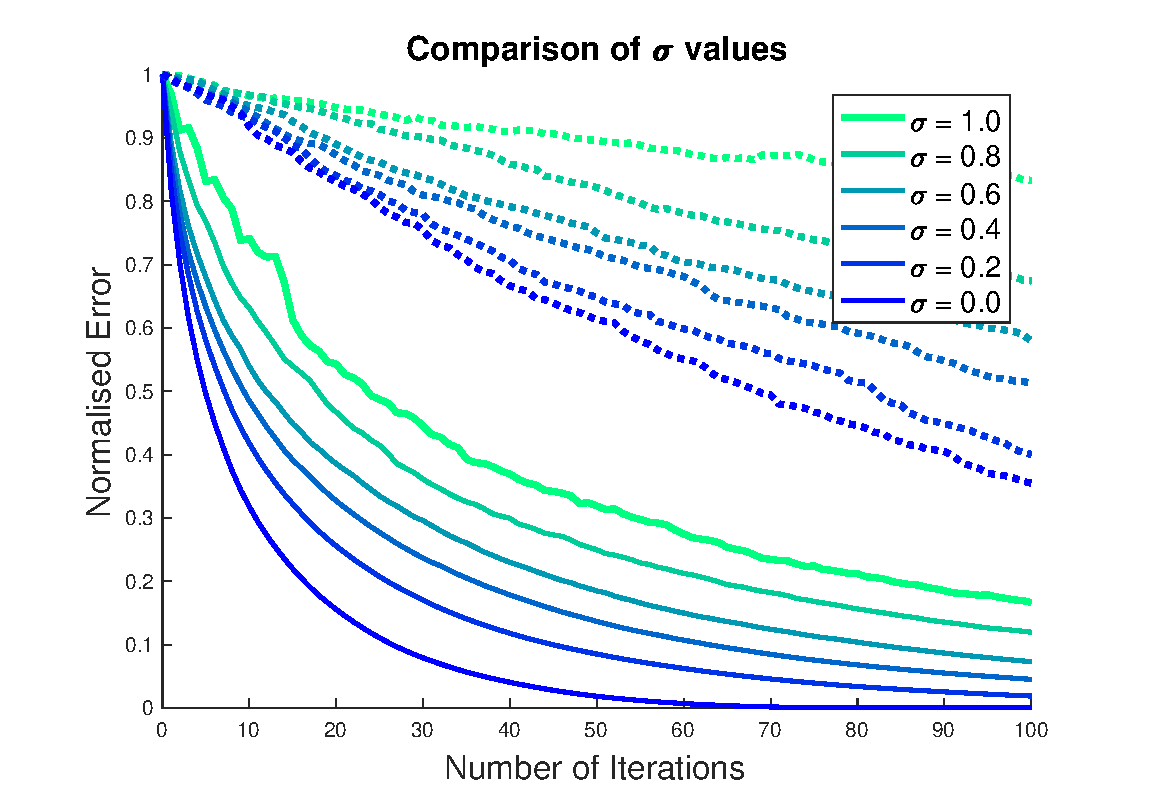
\includegraphics[width = \textwidth/2]{TradInterfaceTests2.eps}
	\caption{Perfect/Imperfect user tests for Traditional Interface}
	\label{fig:TradTest2}
	
	%	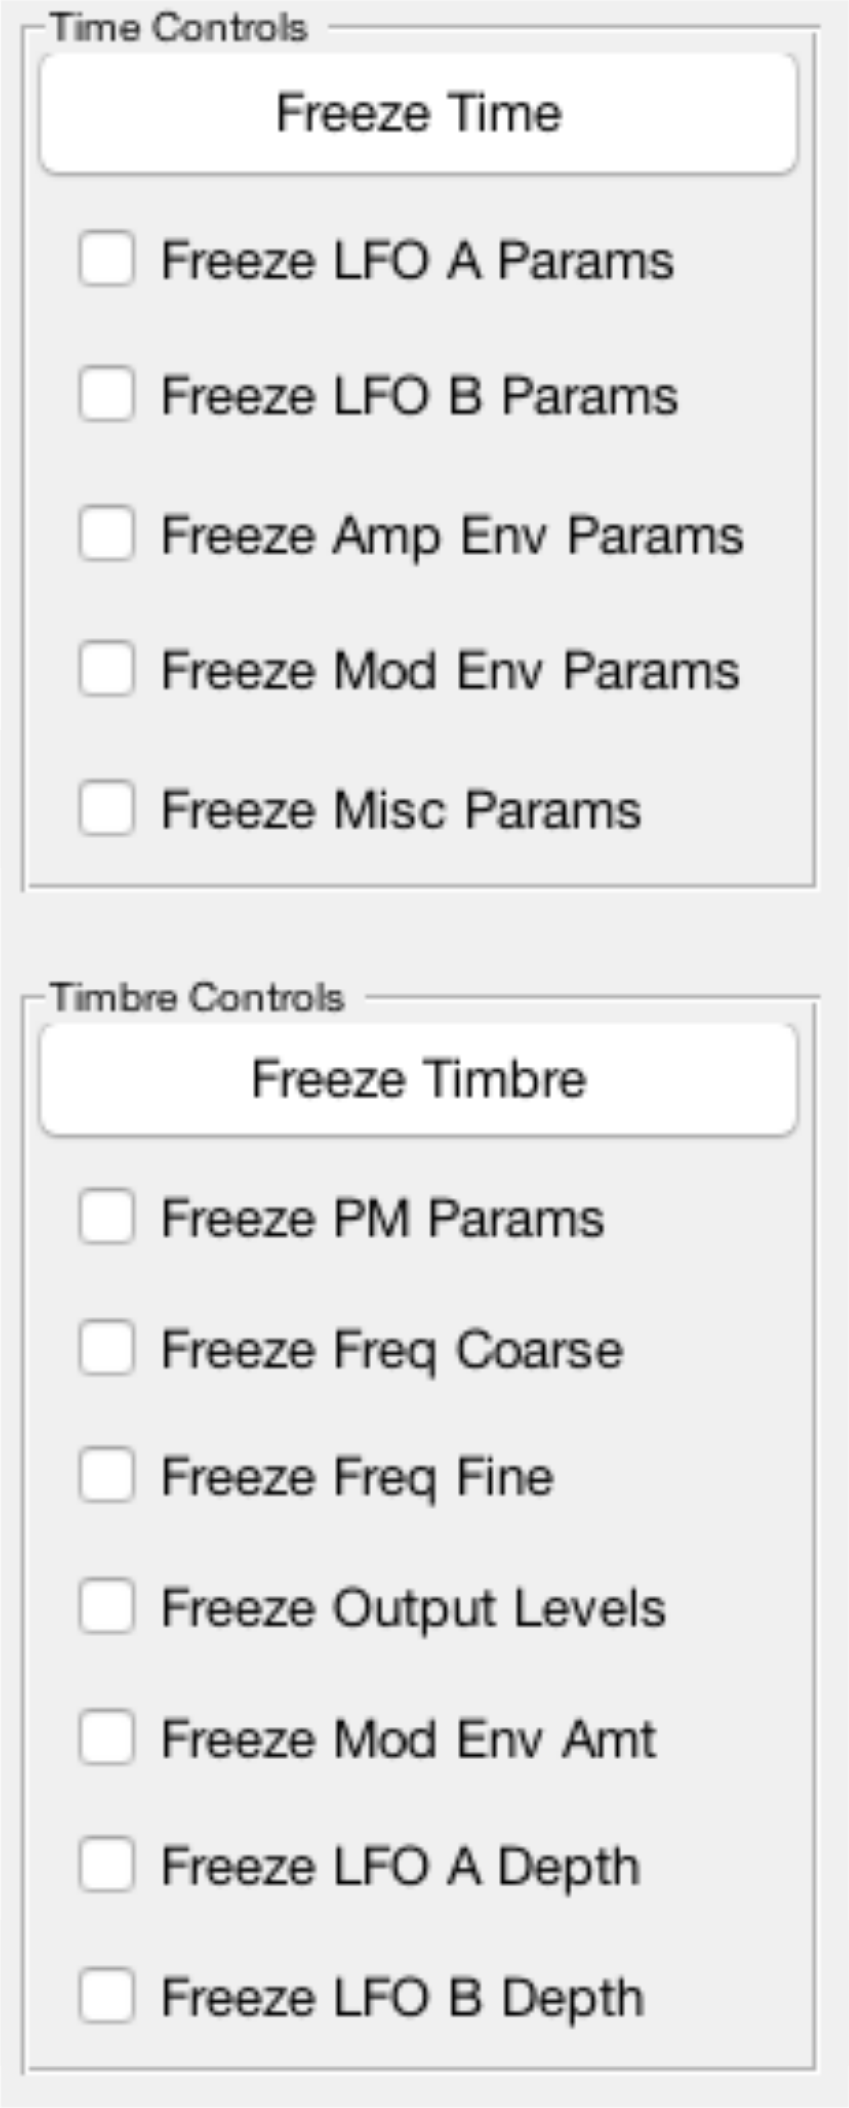
\includegraphics[width = \textwidth/3]{FreezeParams2.png}
	%	\caption{Parameter Freezing}
	%	\label{fig:FreezeParams}
	
%	\vspace{-30pt}
	
\end{figure}

\subsection{Selection Interface}
A similar evaluation was carried out with the selection interface. Again all 36 presets were used as goal presets, with the closest preset used each time as the starting point. For each test, the PCA values were calculated for the remaining 35 presets, simulating the situation where the PCA Macros were being used to find a brand new preset. As before, two parameter orders were tested: the Macro Controls were visited cyclically in order of PCA number, or visited in a random order. For each iteration of the test, the MATLAB 'Patternsearch' search algorithm was used to minimise the cost function for a particular Macro Control. \\ 
A key question with the interface is whether the 'Global' or 'Time/Timbre' version of the PCA Macro Controls should be used. The results for a test with the combination of both sets of macros is shown in Figure \ref{fig:PCAtest1}.
\begin{figure}

\hspace{-60pt}
	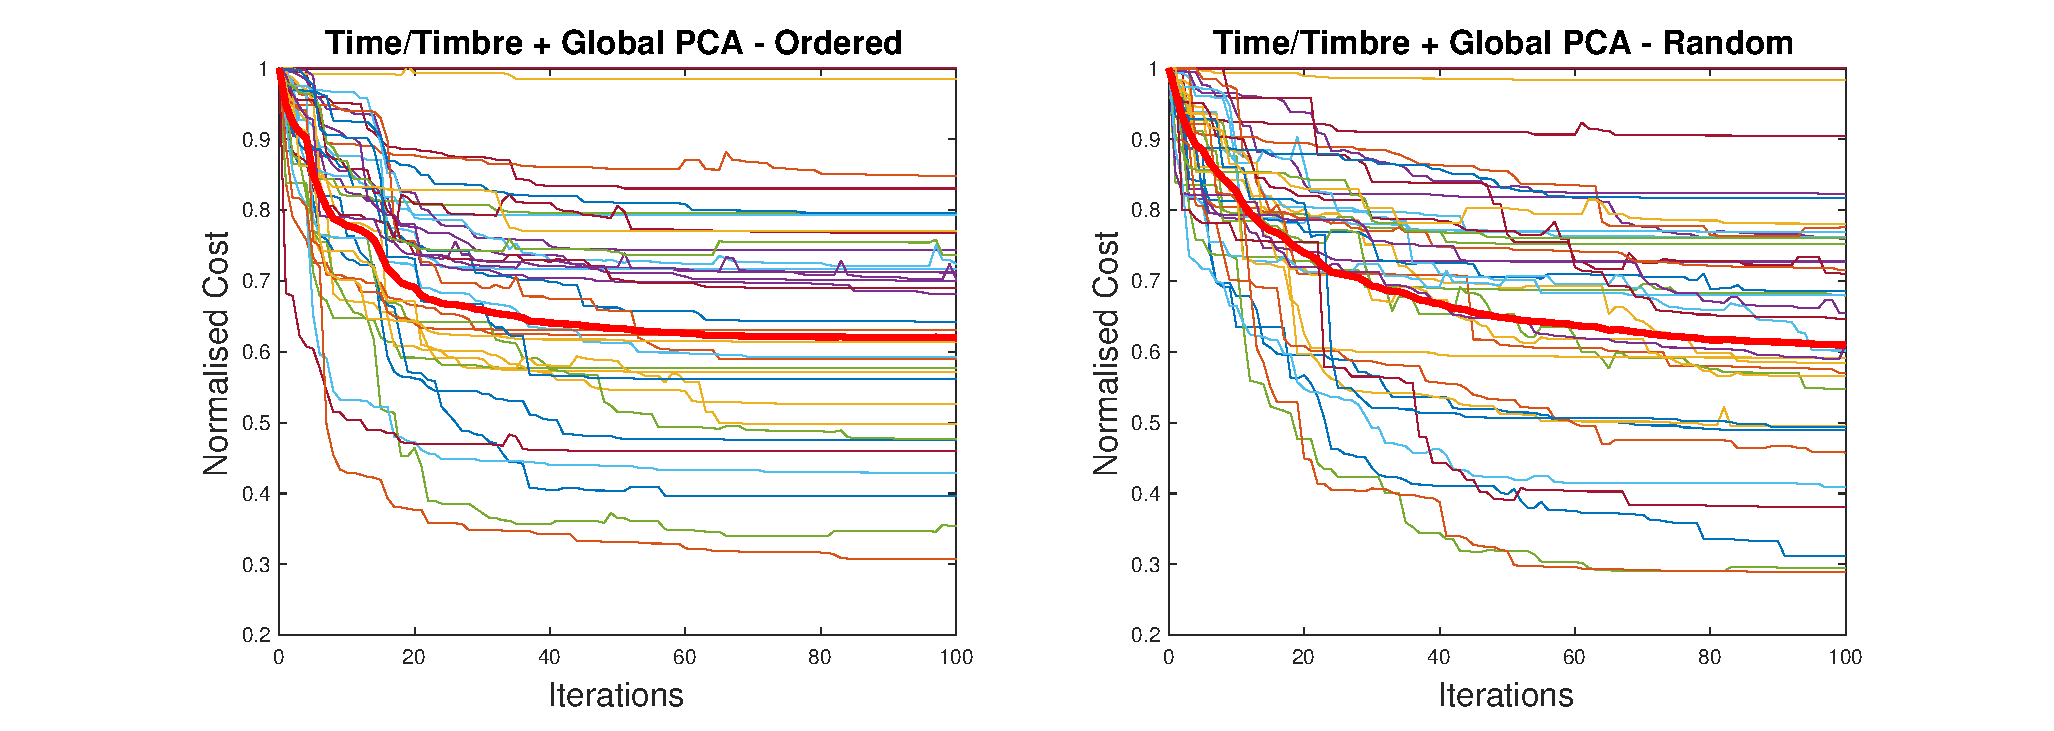
\includegraphics[width = 8in]{PCAInterfaceTests1.eps}
	\caption{Ordered/Random user tests for Selection Interface}
	\label{fig:PCAtest1}
	%	\vspace{-30pt}
\end{figure}

A comparison of the results for the different macro configurations is shown in Figure \ref{fig:PCAtest2}.
\begin{figure}
	\centering
	%	\vspace{-40pt}
	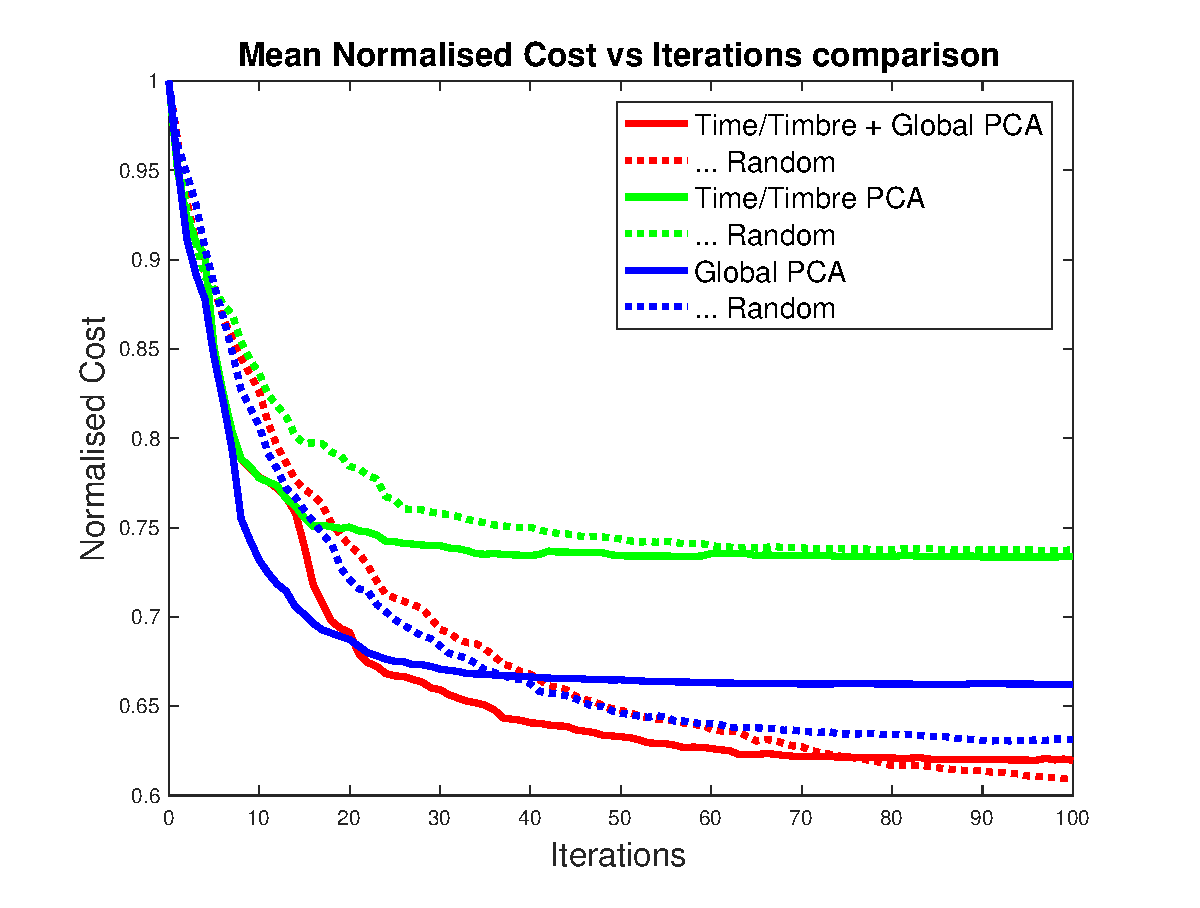
\includegraphics[width = \textwidth]{PCAInterfaceTests2.eps}
	\caption{Comparison of Macro Types}
	\label{fig:PCAtest2}
	%	\vspace{-30pt}
\end{figure}
MAYBE NEED TO DO THE IMPRERFECT USER TESTS ON THE MACRO CONTROLS.

Some points to note from these results:

As shown in Figure \ref{fig:PCAtest1}, for different preset goals, the effictiveness of the PCA Controls varies significantly. In the best case the error drops very rapidly, falling 50\% in the first 10 iterations. In the worst case the error doesn't decrease at all. This suggests that, for this particlar task at least, having the same Macro Controls for each preset may not be ideal, and so a new approach which in some way optimises the Macro Controls per preset would be worth pursuing. However, as previously stated (IN SECTION ????), this comes at the cost of the user being less farmiliar with what the Macro Controls are actually doing. 

In all cases the mean error converges to a non-zero steady state value. This is due to the limited degrees of freedom when using the Macro Controls. This means that the Macro Controls alone cannot be used to prefectly match a goal preset.

When the 'Global' Macro Controls are being used, after a large number of iterations, the random order manages to decrease the error past the cyclic order. It is likely that this is due to the cyclic order getting stuck in a local optimum due to the naive 'one parameter at a time' (BETTER NAME FOR THIS) search algorithm.

Finally, each of the combinations of controls has a similar initial rate of error reduction, but the 'Global' Macro Controls appear to have a significant advantage over the 'Time/Timbre' Macro Controls over larger numbers of iterations. This is likely due to the fact that the Global Macro Controls have access to principal components 1 to 8, whereas the 'Time/Timbre' Macro Controls on have access to two sets of principal components 1 to 4. The combination of both sets of Macro Controls gives the lowest mean error overall, which is unsurprising as it has the most degrees of freedom, and it has a comparable error reduction rate as the 'Global' Controls.

Based on this it is concluded that it is worth keeping both sets of macro controls for the user to be able to select between, especially as the 'Time/Timbre' Macro Controls may lead to more semantically meaningful controls due to the seperation of Time and Timbre. (JUSTIFY THIS MORE)

\subsection{Blending Interface} 
The Blending interface was evaluated in a similar manner. For each of the 36 possible goal presets, the closest three presets to it were found, and these used as preset A, B and C in the blending algorithm. MATLAB's 'Patternsearch' was again used in each iteration to optimise the position of the mouse in the blending interface to minimise the parameter based error metric. 

Results of this test are shown in Figure \ref{fig:BlendingTest1}
\begin{figure}
	%\centering
	\hspace{-70pt}
	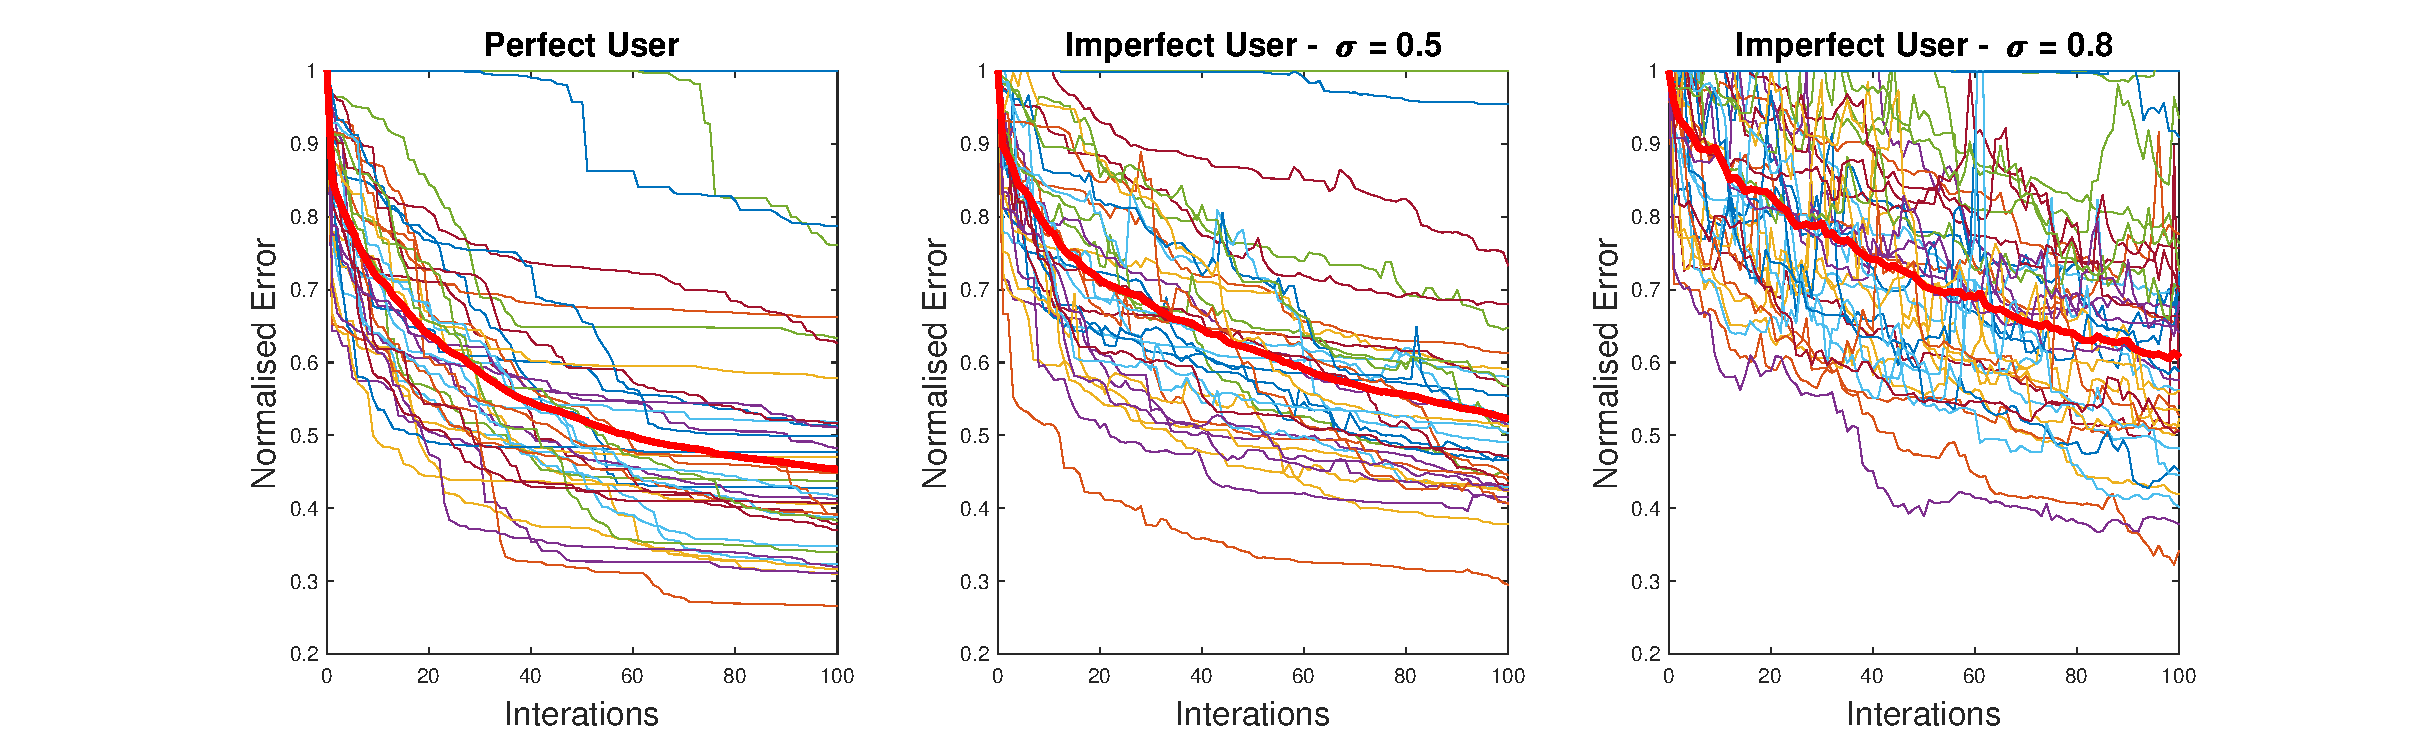
\includegraphics[width = 8in]{BlendingInterfaceTests1.eps}
	\caption{Perfect/Imperfect User tests for Blending Interface}
	\label{fig:BlendingTest1}
	%	\vspace{-30pt}
\end{figure}
On average, there is an rapid decrease in error during the first iteration, followed by an approxiamtely expenential decrease in error.
As in the Selection Interface, there are some tests in which the error barely decreases at all, and some in which the error decreases very quickly, however the variance of the different tests is less than in the PCA interface. For the Perfect User, error is monotoically decreasing, but this is not always the case for the imperfect user, and for real users of the system(EVIDENCE?). This reinforces the need for the Selection History Plot (See Section \ref{sec:BlendingDescription}), which allows users to select several of the local minima in the error plot to resume blending with. (MAYBE MORE DETAIL)

\section{Comparison of combined interfaces}
A comparison of the test results from all three interfaces is shown in Figure \ref{fig:CombinedTest1}. 
\\
The fastest converging test is the Perfect User with Perfect Order on the Traditional Interface, and the slowest converging test is the Imperfect User with Random Order on the Tradtional interface. Interestingly, the order at which the parameters are visited has a much more significant affect than the perfectness of the user. This is due to the Imperfect user model having a zero mean error, so after visiting a parameter several times, the value will converge to the correct value. This result demonstrates that the Traditional Interface can simultaneously be the best possible, and worst possible interface to control a synth with, depending on the experience level of the user, and the intuitiveness of the parameters.

The initial error reduction rate of the Blending Interface is very fast, comparable with the Perfect User of the Traditional interface. The main reason for the initial speed of the blending interface is that in the first iteration, it blends between 3 presets, all close to the goal preset, allowing the first iteration to be a lot less random than subsequent steps. (EXPLAIN BETTER)\\
A key advantage of the Blending Interface is that it removes the need for the user to choose which order to alter the parameters which, as previously described, is the main factor in speed of the Traditional Interface. (MORE DETAIL?)\\
 Over a larger number of iterations, Blending Interface is supassed by the Traditinonal interface with random order. This suggests that the preset generation algoithm is not optimal, as after a while it becomes faster to just sequentially offer the user a random parameter. However, as the user has the option to freeze parameters, and the option to switch to the other interfaces at any point, this may not be an issue. \\
Before converging to their steady state value, the macro controls have quite a fast rate of error reduction - halfway betwen the Perfect User with Perfect or Random Order. This can be partially explained as the Macro Contols allow all of the synthesiser parameters to be varied at once. This also suggests that, as the PCA was carried out on a set of presets, it is likely that the principal components are pointed in a more useful direction than if they'd been selected randomly. (WRITE BETTER)\\
These results suggest that a good workflow for editing synthesis parameters is as follows:
\vspace{-3em}
\begin{itemize}
	\setlength\itemsep{-1.2em}
	\item Find closest 3 presets to desired sound
	\item Use Macro Controls to refine these presets further ($\approx$ 5 iterations per preset)
	\item Use Blending Interface to combine these presets together and further refine ($\approx$ 10 iterations)
	\item Use Traditional interface for final refining of preset. ($\approx$ 20 iterations)
\end{itemize}
\vspace{-0.5em}
The full Interface allows such a process to be carried out, and allows the user to swicth back and forth between the interfaces as often as necessary.

As these tests have only been carried out on one set of presets for one particular synthesiser, an important follow-up work to this project is to validate these results on other synthesisers. As these tests are purely parameter based, the tests could potentially be carried out before doing a full integration of the interface with other synthesisers, as only the set of presets for each synth are needed.

\begin{figure}
	\hspace{-50pt}
	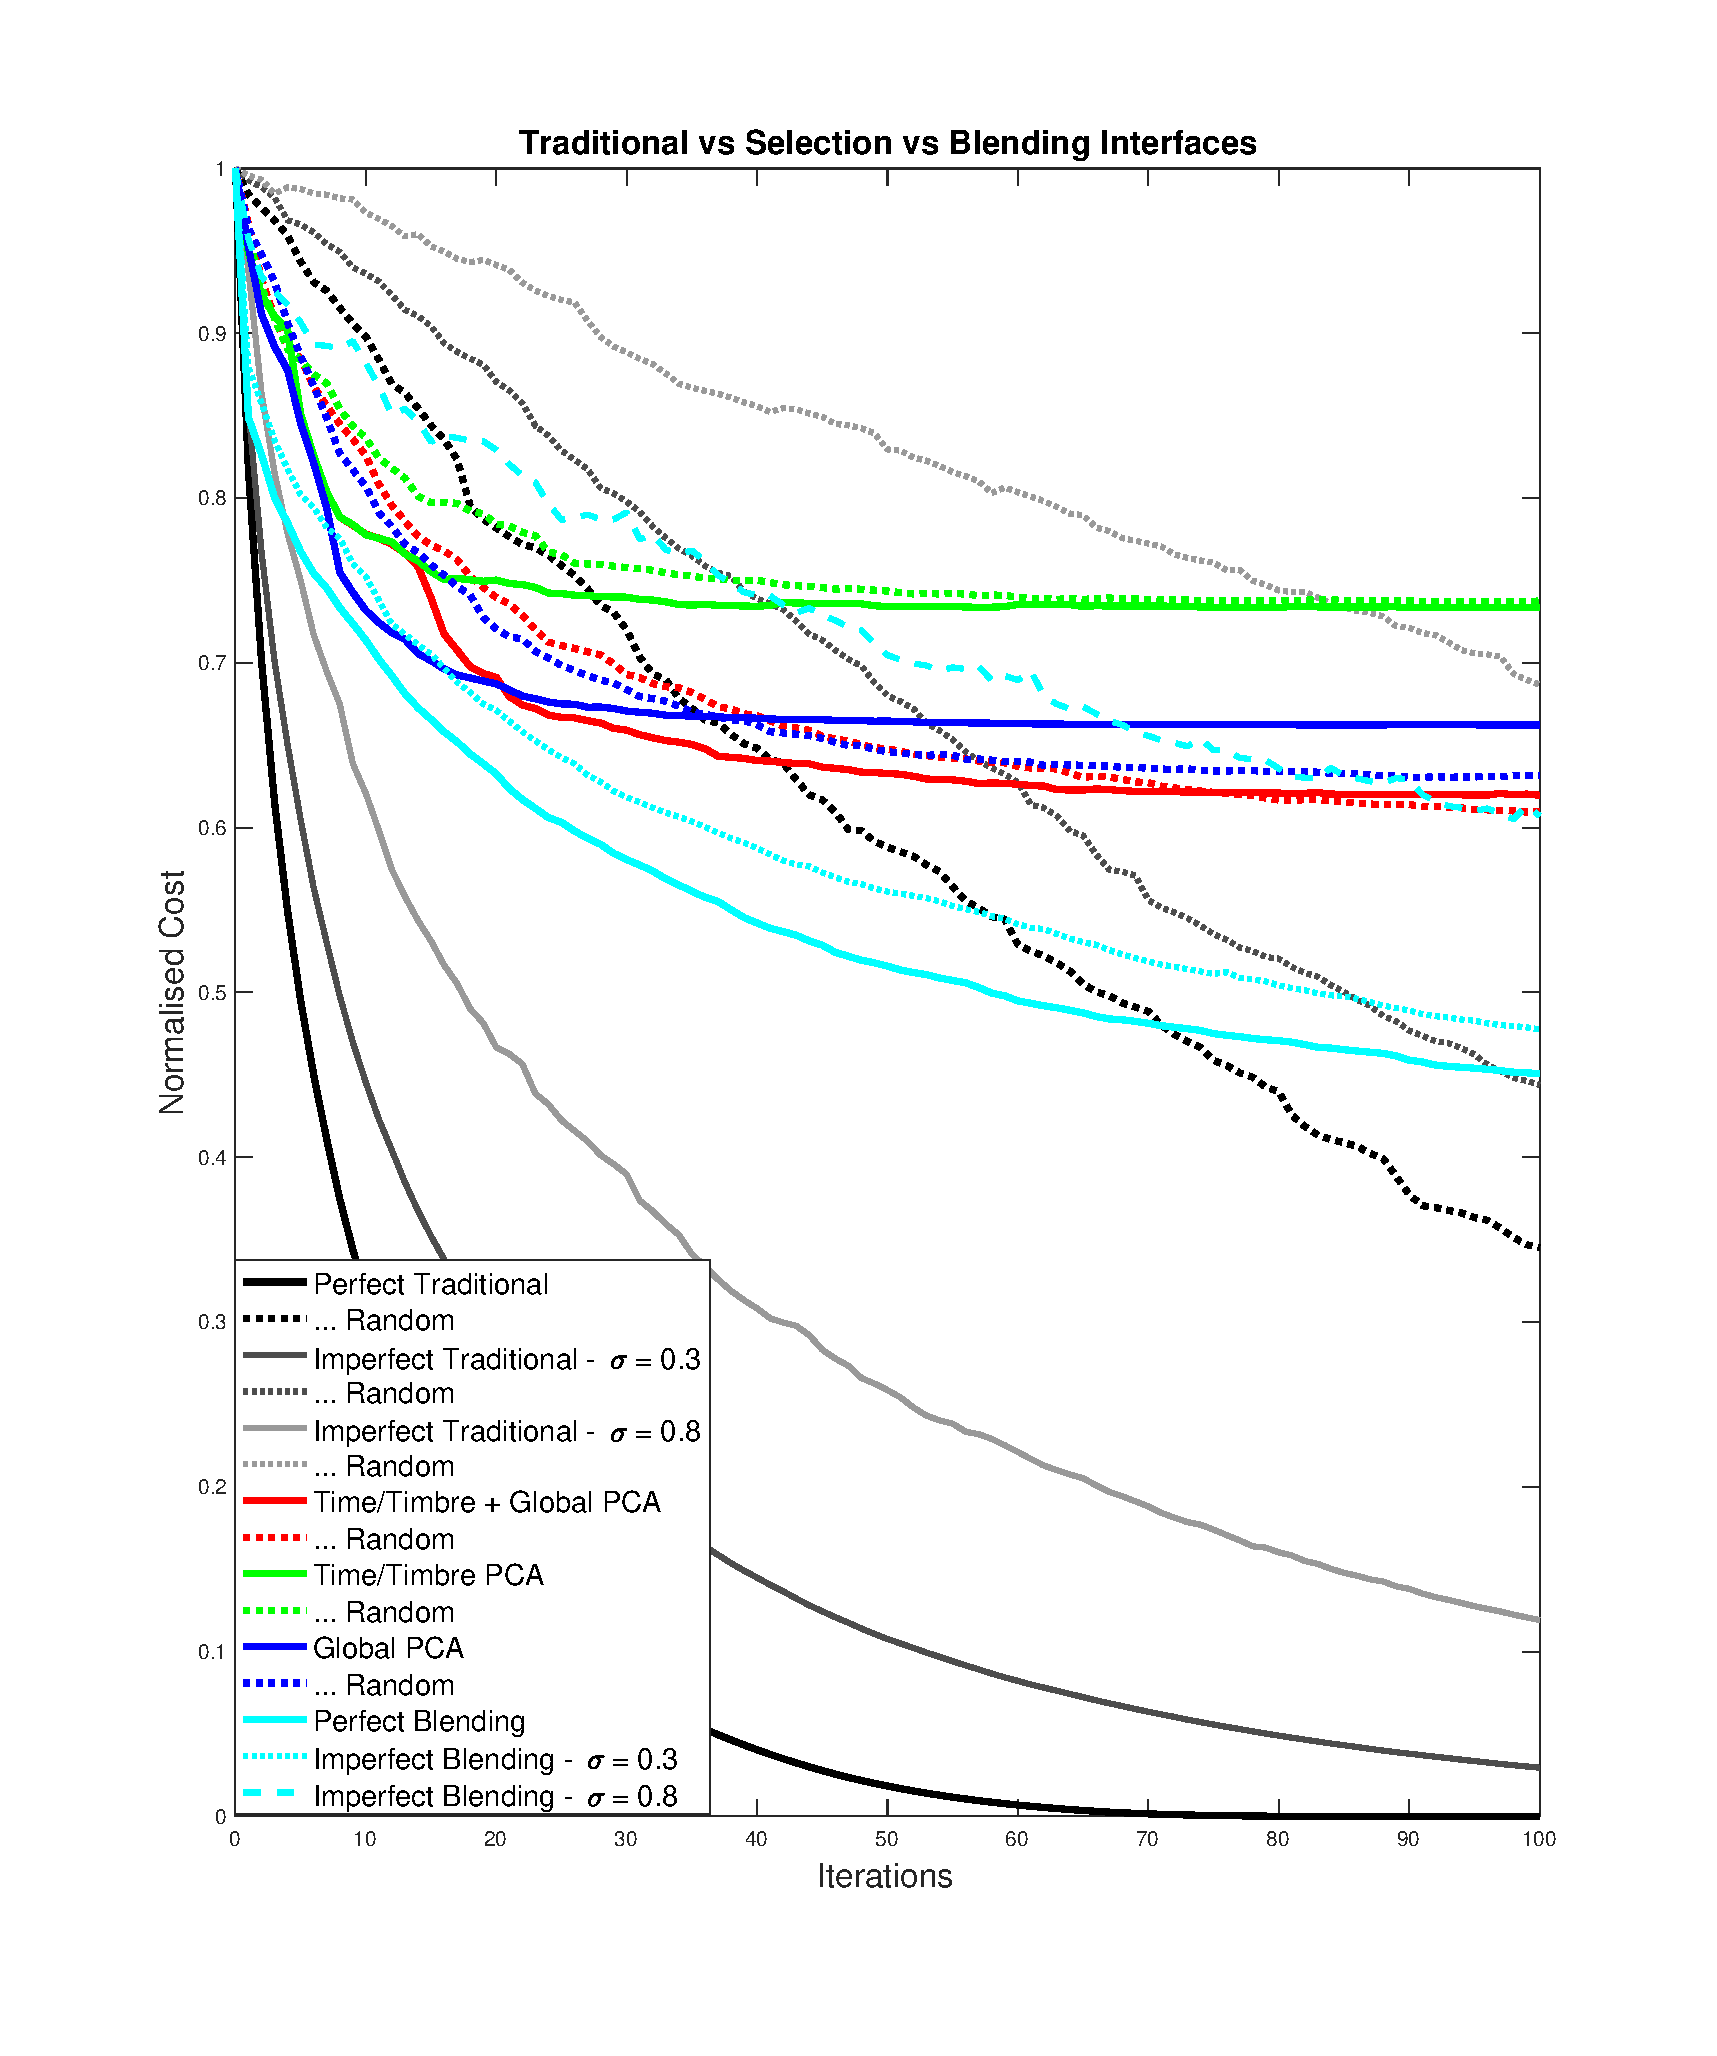
\includegraphics[width = 7.6in]{comparisonOfAllInterfaceGraph3.eps}
	\caption{Comparison of Interfaces}
	\label{fig:CombinedTest1}
	%	\vspace{-30pt}
\end{figure}

\section{EARS-model based evaluation of interface}\label{sec:EARS}
In Table \ref{tab:EARStable}, the three interfaces are evaluated in terms of the EARS model from Section \ref{sec:Tubb} \cite{TubbThesis}.
A conclusion which can be drawn is that the interfaces enables Exploratory, Algorithmic, and Reflective process well, but is not suited to skilled interactions. One of the interfaces could be redisigned with this in mind, or a fourth interface could be introduced.  It should be designed for use with multidimensional controllers, and involve moving through a parameter space consisting solely of the 'nice sounds' of the synthesiser. An Interactive Machine Learning system such as the Wekinator \cite{Wekinator} would be well suited to this task, however more work needs to be done to integrate this approach with the other 3 interfaces.
\begin{table}[h]
	\hspace{-1.5cm}
	\begin{tabular}{|l|l|l|l|l|L|}
		\hline
		\rowcolor[HTML]{EFEFEF} 
		Interface                           & Exploratory? & Algorithmic? & Reflective? & Skilled? & Comments                                                                                                                                                                                                                                                                                                                                                                       \\ \hline
		\cellcolor[HTML]{EFEFEF}Traditional & Maybe        & Yes          & No          & No       & Can be used for exploratory and algorithmic depending on the skill level of the user                                                                                                                                                                                                                                                                \\ \hline
		\cellcolor[HTML]{EFEFEF}Selection   & Yes          & No           & Yes         & No       & \begin{tabular}[c]{@{}L@{}}Exploration by browsing and varying presets. \\ Reflective as easy comparison of presets with combined and varied presets.\end{tabular}                                                                                                                                                                                                            \\ \hline
		\cellcolor[HTML]{EFEFEF}Blending    & Yes          & Maybe        & Yes         & Maybe    & \begin{tabular}[c]{@{}L@{}}Well suited to exploratory, due to simple interface and preset generation. \\ May be used algorithmically due to parameter freezing.\\ The Selection History graph enables reflective comparison and combination.\\ May be used as a skilled strategy, but is not optimised for this approach. Too low dimensional and unpredictable.\end{tabular} \\ \hline
	\end{tabular}
\caption{EARS Model evaluation of synthesiser interfaces}
\label{tab:EARStable}
\end{table}



\chapter{User tests and Interviews}
A rigourous user study would require time and resourses that this project is incapable of, however the interface has been shown to a number of musicians, and some feedback shown below:

NEED TO DO THESE INTERVIEWS
...

\chapter{Conclusion}
The interface proposed in this project has many benefits over a traditional synthesiser interface, as has been designed following design heuristics from the fields of Human Computer Interaction and Creative Cognition. Based on simulated user studies, the interface has at least as good performance as a traditional interface when carrying out search based tasks, and based on real user feedback it has many advantages in terms of creativity. \\
Synthesiser preset datasets are not random, and information can definitely be learned from them. PCA combined with Histogram Equalisation has been identified as a useful dimensionality reduction tool for synthesiser parameters, and several preset generation algorithms have been developed and tested. \\
The interface has also been tested in a different domain, Image Filtering, with promising results. It could easily be applied to many other use cases, such as stage lighting design, or parametric 3D design, as each has a high dimensional parameter set which can be readily controlled over interfaces such as OSC.
\section{Further Work}
The evaluation of this interface was only carried out on a single synthesiser, due to the project's time constraints. An immediate goal is to validate the conclusions from this work on several other synthesisers. The next synthesisers to test should be chosen to include other categories of synthesis, such as Subtractive, Additive and Physical Modelling syntheses. It is non-trivial to extend this work to modular synthesisers, as there is neither a fixed number of parameters, or a fixed achitecture, so different presets may be uncomparable with any common error metric.

The interface has been designed to be as general purpose as possible, allowing it to control arbitrary synths over the OSC protocol, but due to a lack of standardisation between soft synths, and lack of implementation time, more work needs to be done to create a truly general purpose soft synth controller. As many soft-synths are in the Virtual Studio Technology (VST) format, making a version of the interface with acts as a VST Host, and uses the parameter retrieval and preset storage functionality of VSTs is a good next goal if this project is continued in the future.

The interface has been designed with touch-screen contollers in mind, so it would be interesting to implement the interface on a touch screen. Either a dedicated app could be made, or the very customisable OSC controllers Lemur (REFERENCE) or Mira (REFERENCE) could be used. The interface could be further extended by taking into consideration the Multi-Touch capabilities of modern touchscreens.

When the Blending Interface is used, the user carries out a large number of interactions, all of which show a users preference over hyperplanes of parameter settings. If recorded, it may be possible to use these interactions to form a training set to train more sophistocated models of user preference in the parameter space. This can be seen as an extension of the Bayesian Optimisation approach to preference galleries shown in \ref{BayesOptGallery}. As this technique relies on fitting a guassian process to the paramter space, large ammount of training data is necessary, and these interactions may be a way to find such data. As each comparison is choosing the optimum in a hyperplane, as opposed to a binary choice, the interactions have the potentially to be more information dense. Such models of user preference could be used to devise a more sophistocated preset generation algorithm.

Aside from the initial confiuration of presets A, B and C, the Blending Interface currently does not use the preset dataset in its preset generation algorithm. Due to the effectiveness of using this dataset in the Selection Interface, the inclusion of this data is a worthwhile area of further research.

In typical synthesisers, the parameters have a hierarchical nature, as the synthesis algorithm is usally made up of several modules, each with their own parameters and/or sub modules. Many synthesisers store their presets in the JSON (Javascript Object Notation) format, and use such hierarchies to make clean data structures. It may be possible to make use of this hierarchical parameter structure to deduce covariances between parameters, as parameters in the same module are likely to be much more co-dependant than those in seperate modules. Thsi could be used to refine the preset generation and comparison algorithms, and help to detect and correct cases of permutation ambiguity. However this approach has several challenges, most importantly there is a lack of standardisation of preset storage hierarchies.

%The Native Kontrol Standard, is a standardard

\begin{thebibliography}{9}
\singlespacing
\bibitem{UGen}
Stefan Kersten. skUG SuperCollider UGen library., 2008. \url{http://space.k- hornz.de/software/skug/}.

\bibitem{SynthTypes}
Nicol, C. (2005). \emph{Development and Exploration of a Timbre Space Representation of Audio}. Ph.D. University of Glasgow.

\bibitem{TubbThesis}
Tubb, R. (2016). \emph{Creativity, Exploration and Control in Musical Parameter Spaces}. Ph.D. Queen Mary University of London.

\bibitem{YeeKing}
Yee-King, M. (2011). \emph{Automatic Sound Synthesizer Programming: Techniques and Applications}. Ph.D. University of Sussex.
\end{thebibliography}
\end{document}  